\chapter{How graphene slides: Measurement and theory of strain-dependent frictional forces between graphene and $\mathrm{SiO_2}$}

Graphene is an amazing mechanical system with extreme elasticity\cite{Lee2008}, ultrastrong adhesion\cite{Koenig2011}, and impermeability to gases\cite{Bunch2008}.  As a pure two dimensional material, graphene's interactions with its supporting substrate are unique.  Amontons' first law states that macroscopic friction is proportional to the applied load, justified by arguing that increasing the load increases the microscopic contact area between two surfaces\cite{Krim1996}.  Graphene, however, because of its ultrastrong adhesion\cite{Koenig2011} and low bending rigidity requires no load to achieve nearly perfect conformation to the nanoscale topography of its substrate, especially the commonly used $\mathrm{SiO_2}$\cite{Stolyarova2007,Lui2009,Cullen2010}.  Hence, the friction between graphene and $\mathrm{SiO_2}$ might be expected to exhibit an atypical load dependence. The ability to control the thickness of few layer graphene (FLG) at an atomic scale makes it an excellent model system to study the role of thickness and load on friction, which has not previously been quantified or elucidated in detail.  To date most tribological studies of FLG and graphitic materials have measured the interaction between graphene and a scanning probe tip using frictional force microscopy\cite{Dienwiebel2004,Deng2012,Lee2010,Li2010c,Filleter2009,Filleter2010,Zhang2012a}.  These nanoscale measurements have shown interesting effects such as superlubricity in graphite\cite{Dienwiebel2004}, negative frictional coefficient for chemically modified graphite\cite{Deng2012}, and increasing friction with decreasing FLG thickness\cite{Lee2010,Li2010c,Filleter2009,Filleter2010}.  Both the negative frictional coefficient and the increasing friction with decreasing thickness have been attributed to the puckering of graphene about the scanning probe tip\cite{Lee2010,Li2010c,Deng2012}.

Here, for the first time, we directly measure the intrinsic sliding of graphene over a $\mathrm{SiO_2}$ substrate at the macroscopic device scale and, further, extract both the load and atomic layer dependence of sliding friction, or the substrate's resistance to graphene sliding.  We isolate the graphene-substrate interaction and avoid introducing a scanning probe tip to the system by using variable gas pressure applied to an FLG sealed microchamber as shown in Figure \ref{device}.  The pressure acts as a tunable load, simultaneously pressing the supported graphene into the substrate while forcing the suspended FLG into the microchamber.  \emph{In situ} Raman measurements, which can easily measure FLG extensions of $1 \ nm$ over $1 \ \mu m$, show that an annulus of the supported FLG reproducibly slides toward the center of the microchamber.  By analyzing the strain response with a newly derived extension of the continuum Hencky model, we are able to extract load-dependent sliding frictions for mono-, bi-, and tri-layer graphene.  The layer dependence exhibits a crossover between bilayer and trilayer; the trilayer sliding friction obeys Amontons' first law, whereas the monolayer and bilayer sliding friction uniquely scales with the inverse of the strain in the graphene.  We attribute these interesting results to the interplay between adhesion, in-plane strain and bending rigidity in this two dimensional tribological system.  A firm understanding of graphene's sliding friction is necessary for a variety of exciting graphene devices such as flexible bistable displays\cite{Bonaccorso2010}, graphene electro-mechanical switches\cite{Milaninia2009}, strain engineered devices\cite{Pereira2009a} which take advantage of strain induced vector-potentials and pseudomagnetic fields\cite{CastroNeto2009,Guinea2009,Kitt2012}, and high quality factor graphene mechanical resonators\cite{Kim2009,Bunch2007,Chen2009,Barton2011}.

\begin{figure}
\begin{center}
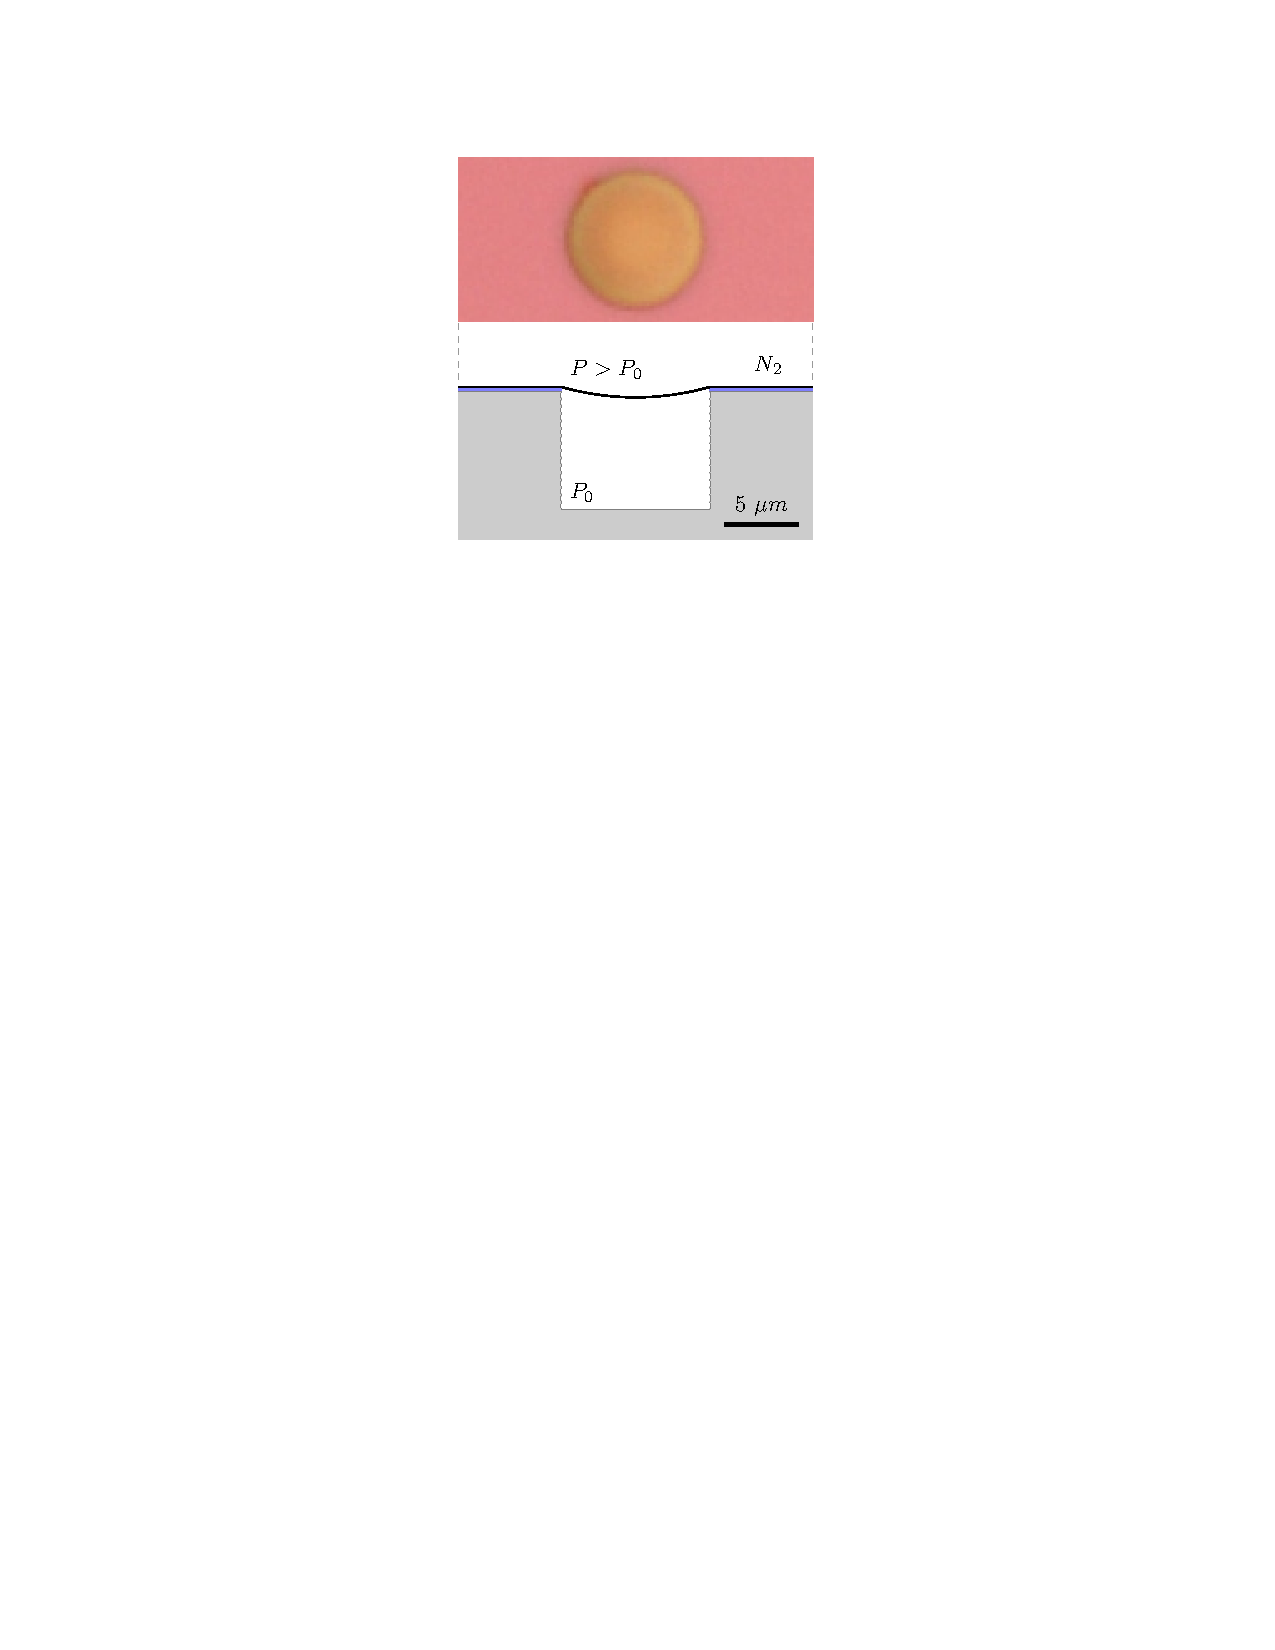
\includegraphics{Figs_Friction/Figure_1.pdf}
\end{center}
\caption{\label{device} Top: An optical image of a trilayer graphene-sealed microchamber. Bottom: Device cross-section schematic showing the microchamber etched $8 \ \mu m$ into the underlying Si substrate and the supported graphene atop the 300 nm of thermal oxide.  Pictured to scale is the largest pressure induced deflection of the graphene achieved in any of the analyzed experiments.}
\end{figure}

\section{Raman G band strain response}
Micro-Raman spectroscopy is a powerful tool to measure strain distributions in graphene.  The Raman G band measures the zone center, in-plane optical phonons that are degenerate at zero strain.  In the absence of shear strain, the G band shifts according to\cite{Huang2009}:
\begin{equation}
\Delta \omega_G=-\omega_0 \gamma(\epsilon_{r}+\epsilon_{t}) \pm \frac{1}{2} \beta (\epsilon_{r}-\epsilon_{t})
\end{equation}
where $\epsilon_{r}$ and $\epsilon_{t}$ are the strain in the radial and tangential directions,  $\gamma$ is the Gr\"{u}neisen parameter and $\beta$ is the shear deformation potential which details the amount of splitting between the $G^+$ and $G^-$ bands.  Light scattered by the $G^+$ and $G^-$  bands has orthogonal linear polarizations\cite{Huang2009}.  Unless otherwise noted, circularly polarized light is used so that the $G^+$ and $G^-$ bands are measured simultaneously.  Figure \ref{circlelinear} shows that the spectra taken using circular polarized light match the sum of the $G^+$ and $G^-$ bands which were measured using linearly polarized light.

\begin{figure}
\begin{center}
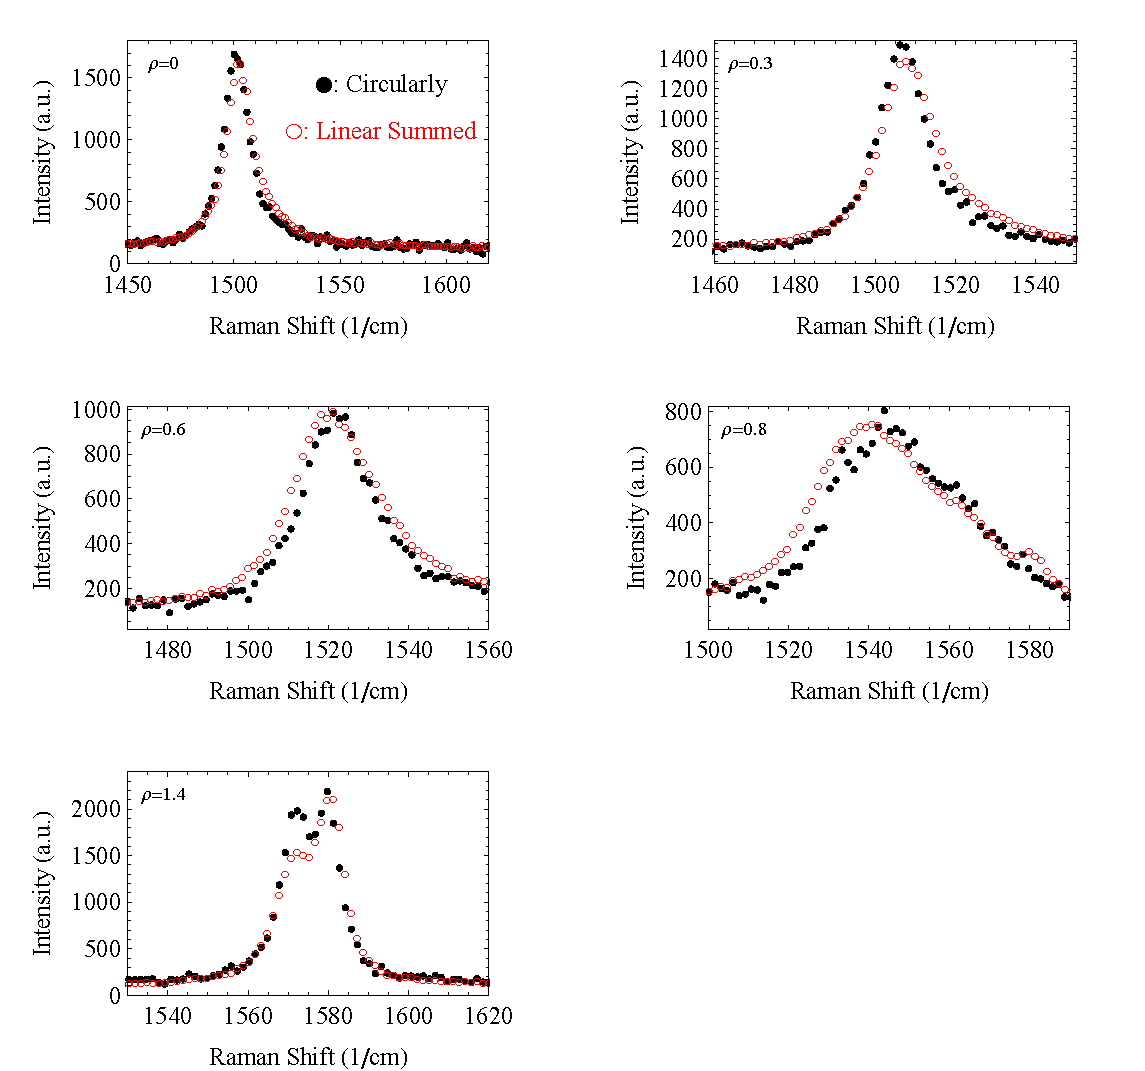
\includegraphics[scale=.75]{Figs_Friction/LinearvsCircular.pdf}
\end{center}
\caption{\label{circlelinear}A comparison of Raman spectra measured using circularly and linearly polarized light. Measurements were taken at the labeled positions on a $5 \ \mu m$ radius graphene sealed microchamber with 0.80 MPa of applied absolute pressure. The black dots show the spectrum measured using circularly polarized light while the red dots are the sum of the spectra taken with incident polarization set in the $\hat x$ direction and outgoing polarization analyzed from -90 to 90 degrees in 20 degree steps.  The spectra are scaled to match intensities. Thus, the red dots give the signal from both the $G^+$ and $G^-$ bands measured in the standard linearly polarized way.  The agreement between the red and black dots proves that the measured circularly polarized spectra simply give the sum of the contributions from the $G^+$ and $G^-$ peaks.}
\end{figure}

The local Raman response is measured inside an optically accessible pressure chamber with a focused laser beam while variable pressures up to 0.80 MPa are used to push the FLG into the microchamber.  Raman spectra are excited using the 514 nm line of an argon ion laser and collected using a Renishaw spectrometer with an 1800 lines/mm grating and a 63X, .7 NA, cover slip corrected objective.  The laser power in the pressure chamber was kept below 0.5 mW to avoid sample heating.  The optical access in the pressure chamber is through a 1 mm BK7 window.  The beam waist of the focused laser was measured to be $0.83 \pm .01 \ \mu m$ by scanning a gold pad under the laser as shown in Figure \ref{waist}.

\begin{figure}
\begin{center}
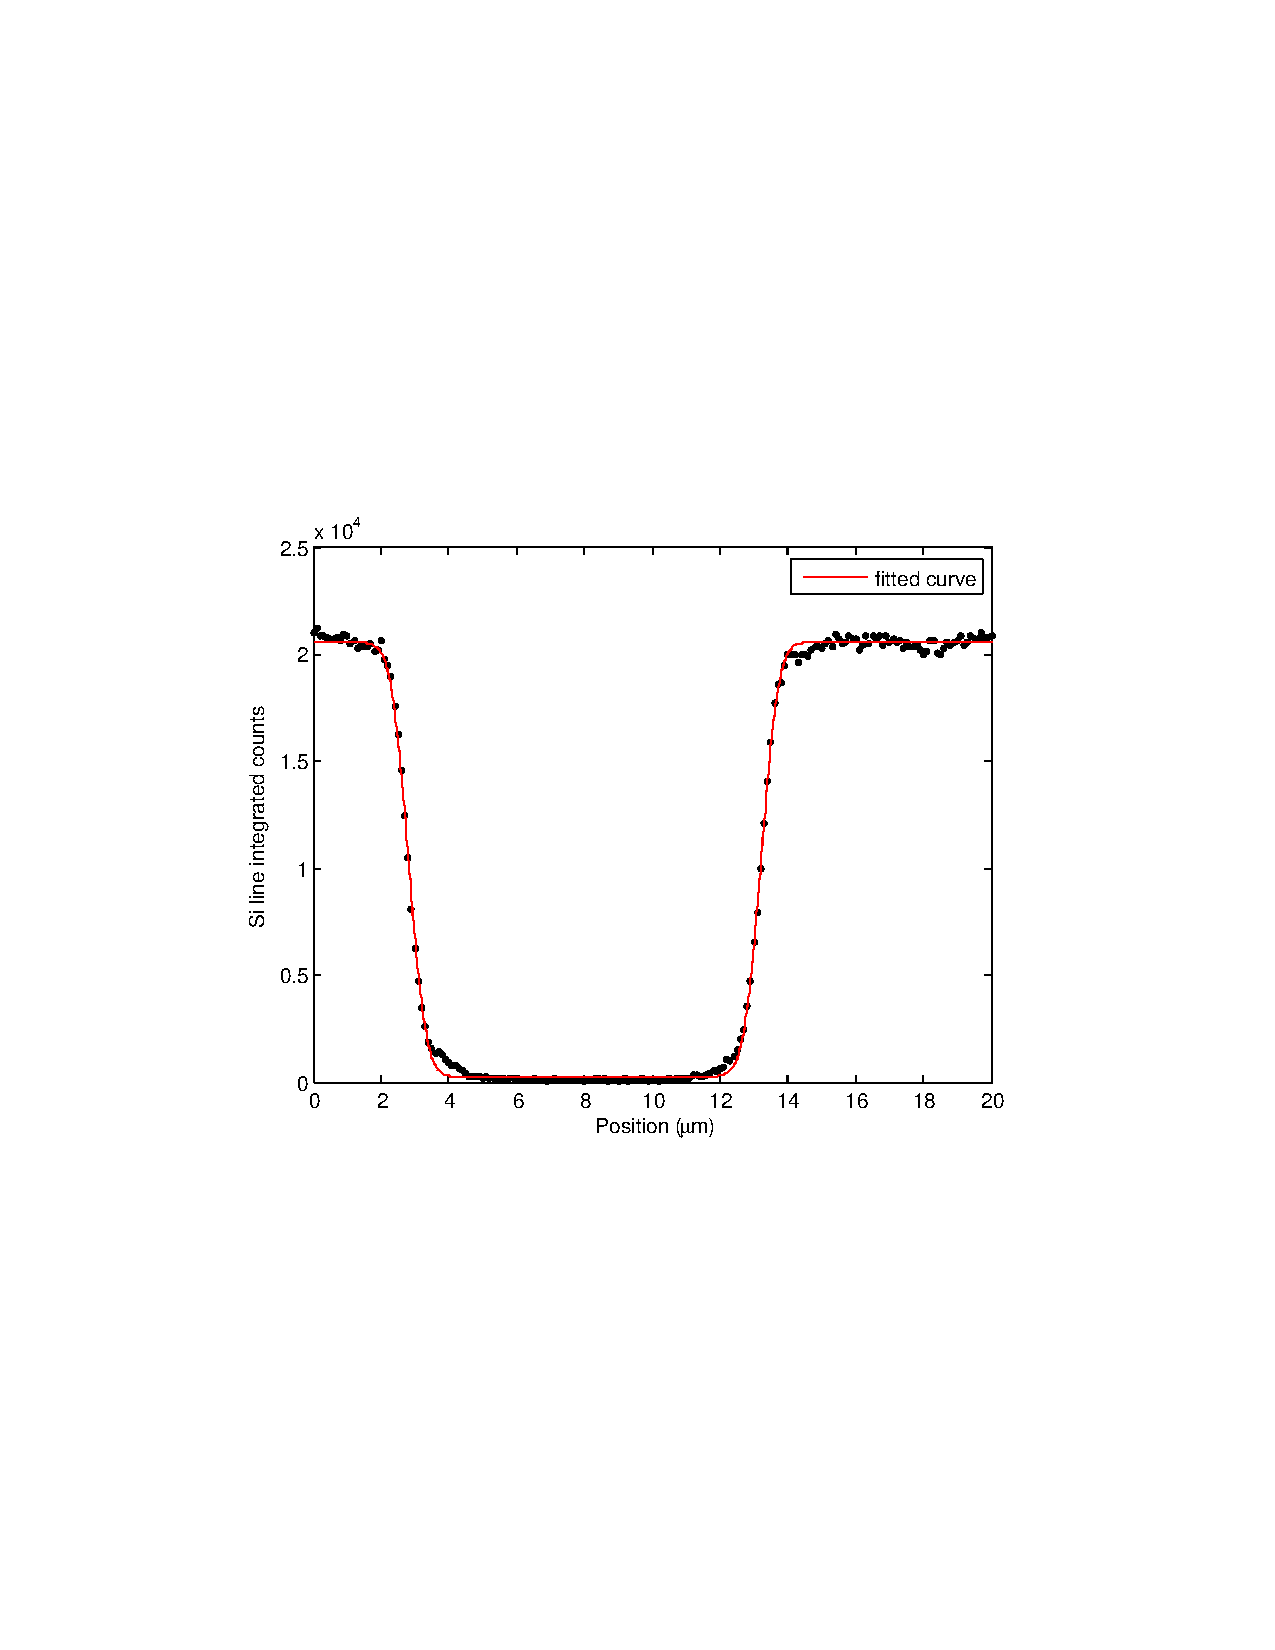
\includegraphics[scale=1]{Figs_Friction/SpotSize.pdf}
\end{center}
\caption{\label{waist}Determination of the beam waist of the focused laser in the pressure chamber. A sample with a gold pad was scanned under the focused beam while measuring the Si Raman line intensity. As the sharp edge of the gold pad moves under the laser, the Si line is blocked giving a measure of the beam size. Fitting the signal to an error function gives a beam waist of $0.81 \pm .01 \ \mu m$.}
\end{figure}

\section{Experimental Design}
A cross-section of one of our microchambers sealed with mechanically exfoliated FLG is depicted in Figure \ref{device}. Microchambers are fabricated using standard optical lithographic methods to define holes ranging from 1 to 5 $\mu m$ in radii,  reactive ion etching to etch through the 300 nm thermal oxide layer, and deep reactive ion etching to etch roughly $8 \ \mu m$ into the underlying silicon layer.  Before the graphene is mechanically exfoliated to seal the microchambers, the substrate is oxygen plasma ashed for 10 minutes at 300 sccm and 500 Watts to ensure the substrate is cleaned of any residues. The number of graphene layers sealing each device was determined using Raman spectroscopy\cite{Ferrari2006} and optical contrast\cite{Blake2007,Casiraghi2007a}.

The large microchamber depth of $\sim 8 \ \mu m$ is 10 times the largest FLG deflection of $700 \ nm$, allowing us to both ignore changes in internal pressure as the applied pressure is increased, and to measure for longer times because of slower leak-out rates through the silicon substrate.  To eliminate surface residues, the substrate was oxygen plasma ashed before FLG exfoliation. It is important to note that different surface treatments may yield different sliding frictions providing a new degree of freedom in device engineering. 

Two complementary Raman measurements are performed \emph{in situ} to fully characterize the strain distributions. First, as the absolute applied pressure is varied between atmospheric pressure (0.10 MPa) and 0.80 MPa, Raman spectra at the center of the microchamber are recorded. Also, at selected pressures, Raman G band line scans with $ 0.5 \ \mu m$ point spacing are taken across the microchamber.  The former is used to determine the pressure inside of the microchamber while the latter is used to determine the spatial distribution of the strain.  In conjunction with low force ($\approx 1 \ nN$) contact mode atomic force microscopy (AFM), the Raman spectra taken at the center of the microchamber reveal interesting ambient pressure behavior exhibited by the graphene sealed microchambers.

\subsection{Characteristic ambient pressure behavior of FLG sealed microchambers}
The ambient pressure behavior of the measured devices is split roughly evenly between two representative cases. For half of the devices the pressure inside of the microchamber was greater than ambient, as shown in the left side (a) of Figure \ref{ambient}.  Here, both the AFM and Raman measurements indicate that the pressure inside of the microchamber is greater than ambient. The topographic image shows the graphene bulging out and the Raman G band response demonstrates that a non-zero gauge pressure is necessary for the G band to reach its greatest, or least strained, value. By fitting the Raman data with the $p^{2/3}$ form predicted by the standard Hencky model for the strain at the center of the hole (blue dashed line), the internal pressure and unstrained peak position are found. In the second half of the devices, the pressure inside the microchamber was an atmosphere, as shown on the right side (b) of Figure \ref{ambient}.  The AFM topography shows that the graphene is flat across the aperture indicating the internal pressure matches the ambient pressure. The graphene is also stuck down to the wall edges for an AFM determined distance of roughly $7 \ nm$.  Other groups have observed similar snap-to-sidewall behavior\cite{Lee2008,Bunch2008}. Bunch and Dunn noted that the AFM measured distance over which FLG snaps to sidewalls may be overestimated\cite{Bunch2012}, a position supported by our Raman measurements of the strain in these devices.  Additionally, the Raman G band response in these devices shows interesting small strain behavior with increasing pressure which we believe to be a result of graphene peeling off the edge of the walls. At atmospheric pressure the G band is already red shifted due to pre-strain. Increasing the gauge pressure to $\sim 0.1$ MPa causes a slower than expected downshift in the G band position. However, when the gauge pressure is increased beyond $0.1$ MPa, the shift rate converges to the expected trend, $P^{2/3}$, and remains on this trend when the pressure is reduced back to atmospheric pressure.  We believe this is a signature of the FLG unsticking from the walls as pressure is applied and may explain the small Young's Modulus measured by Lee \emph{et al.} using a similar measurement over the a 0.1 MPa pressure range\cite{Lee2012}.

\begin{figure}
\begin{center}
	\newcommand{\xs}{4.5 cm}
	\newcommand{\totscale}{.6}
	\newcommand{\afmscale}{.42}
	\begin{tikzpicture}[scale=\totscale]
		%SB02-3
		\begin{scope}[xshift=\xs]
			\node at (0,0) {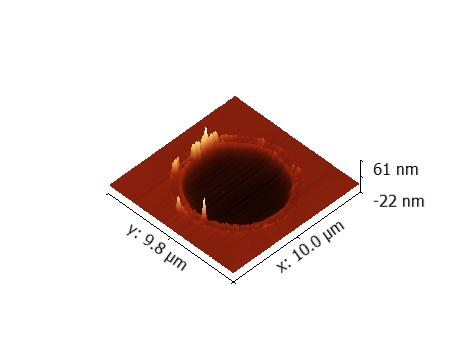
\includegraphics[scale=\afmscale]{Figs_Friction/AFM_SB02-3.jpg}};
			\node at (0,-4.5 cm) {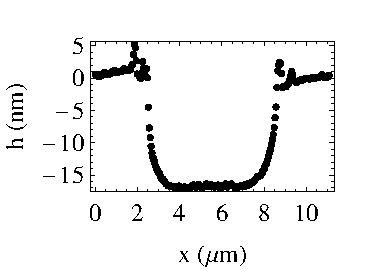
\includegraphics[scale=\totscale]{Figs_Friction/Section_SB02-3.pdf}};
			\node at (0,-10 cm) {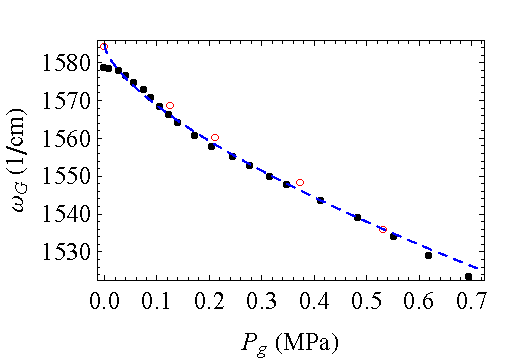
\includegraphics[scale=\totscale]{Figs_Friction/CenterFit_SB02-3.pdf}};
		\end{scope}
		%SB03-2b
		\begin{scope}[xshift=-\xs]
			\node at (0,0) {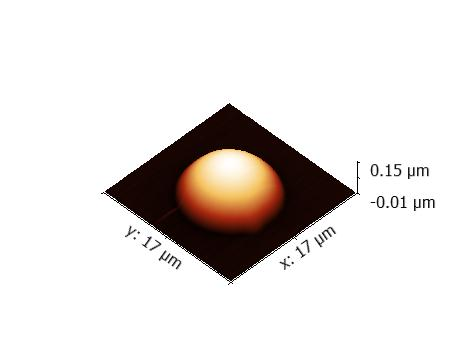
\includegraphics[scale=\afmscale]{Figs_Friction/AFM_SB03-2A.jpg}};
			\node at (0,-4.5 cm) {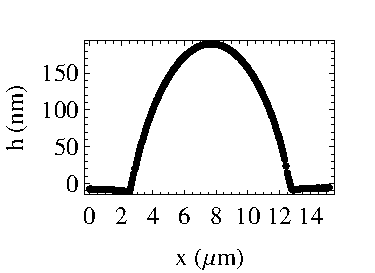
\includegraphics[scale=\totscale]{Figs_Friction/Section_SB03-2A.pdf}};
			\node at (0,-10 cm) {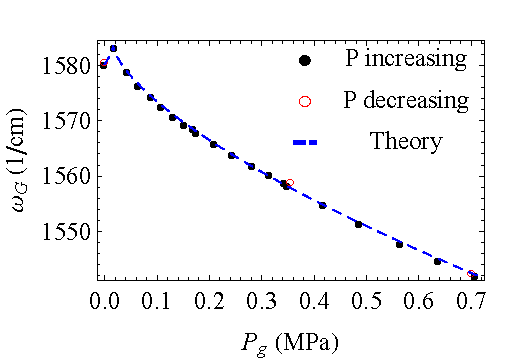
\includegraphics[scale=\totscale]{Figs_Friction/CenterFit_SB03-2A.pdf}};
		\end{scope}
		
		\node at (.7,1.75) [anchor=south west]{\textbf{b}  Snapped to side wall};
		\node at (-8,1.75) [anchor=south west]{\textbf{a} $P_0>P_a$};
	\end{tikzpicture}
\end{center}
\caption{Characteristic ambient pressure behavior of FLG sealed microchambers. Low contact force ($\approx 1\ nN$) AFM taken at ambient pressure with line cuts (top) and the center frequency of the single Lorentzian fit spectra taken at the center of the hole as a function of the applied gauge pressure (bottom) for (a) (left hand side) a $10 \ \mu m$ trilayer sealed microchamber and (b) (right hand side) a $6 \ \mu m$ monolayer sealed microchamber.\label{ambient}}
\end{figure}

\section{Qualitative results}
The Raman line scans over pressurized microchambers show that the supported graphene around the microchamber has slid inward toward the center.  Figure \ref{qualresults} shows the G band center frequency of the fit Lorentzians plotted as a function of position across a $6 \ \mu m$ diameter monolayer covered graphene sealed microchamber with applied absolute pressures of 0.45 and 0.80 MPa during three separate pressure cycles from atmospheric to 0.80 MPa. As expected, as the suspended graphene is pushed down into the microchamber, the G band red shifts or softens from its unstrained value.  Unexpectedly, the G band of the supported graphene \emph{outside} the edge of the microchamber also shows softening, and thus significant strain.  The observed softening decreases with the distance from the edge of the microchamber until the G band returns to its unstrained energy.  This strain is real; the G band red shift cannot be attributed to the averaging over the finite spot size of the beam because the measured downshifts persist much further from the edge of the microchamber than the $0.83 \ \mu m$ beam waist. As the applied pressure increases, more strain is distributed outside of the microchamber causing both a larger redshift and a larger region over which the strain is distributed.  The strain distributed outside of the microchamber's edge is a clear indicator that the graphene is not rigidly fixed to the substrate outside of the microchamber.  Instead of a line force acting at the circumference of the microchamber to fix the graphene at the edge, there must be a distributed sliding frictional force, $f$, acting between the graphene and the substrate.

This behavior is reproducible, stable, and azimuthally symmetric.  The four 0.45 MPa line scans in Figure \ref{qualresults} include one line scan in the x direction for each of the first two pressure cycles and a line scan from both the x and y direction during the third pressure cycle.  The five 0.80 MPa line scans include one line scan in the x direction from the first pressure cycle, two sequential line scans in the x direction which took 35 minutes each from the second pressure cycle, and a line scan from both the x and y direction during the third pressure cycle.  Other than the development of a dimple at the center of the microchamber, the spectra and G band shifts are nearly identical.  This dimple is the result of laser deposition of dirt at the center of microchamber due to tens of hours of high pressure resolution, single point measurements.  This dirt seems to stabilize the graphene underneath, reducing the strain in its vicinity.  An SEM image of the schmutz dimple is shown in the inset.

\begin{figure}
\begin{center}
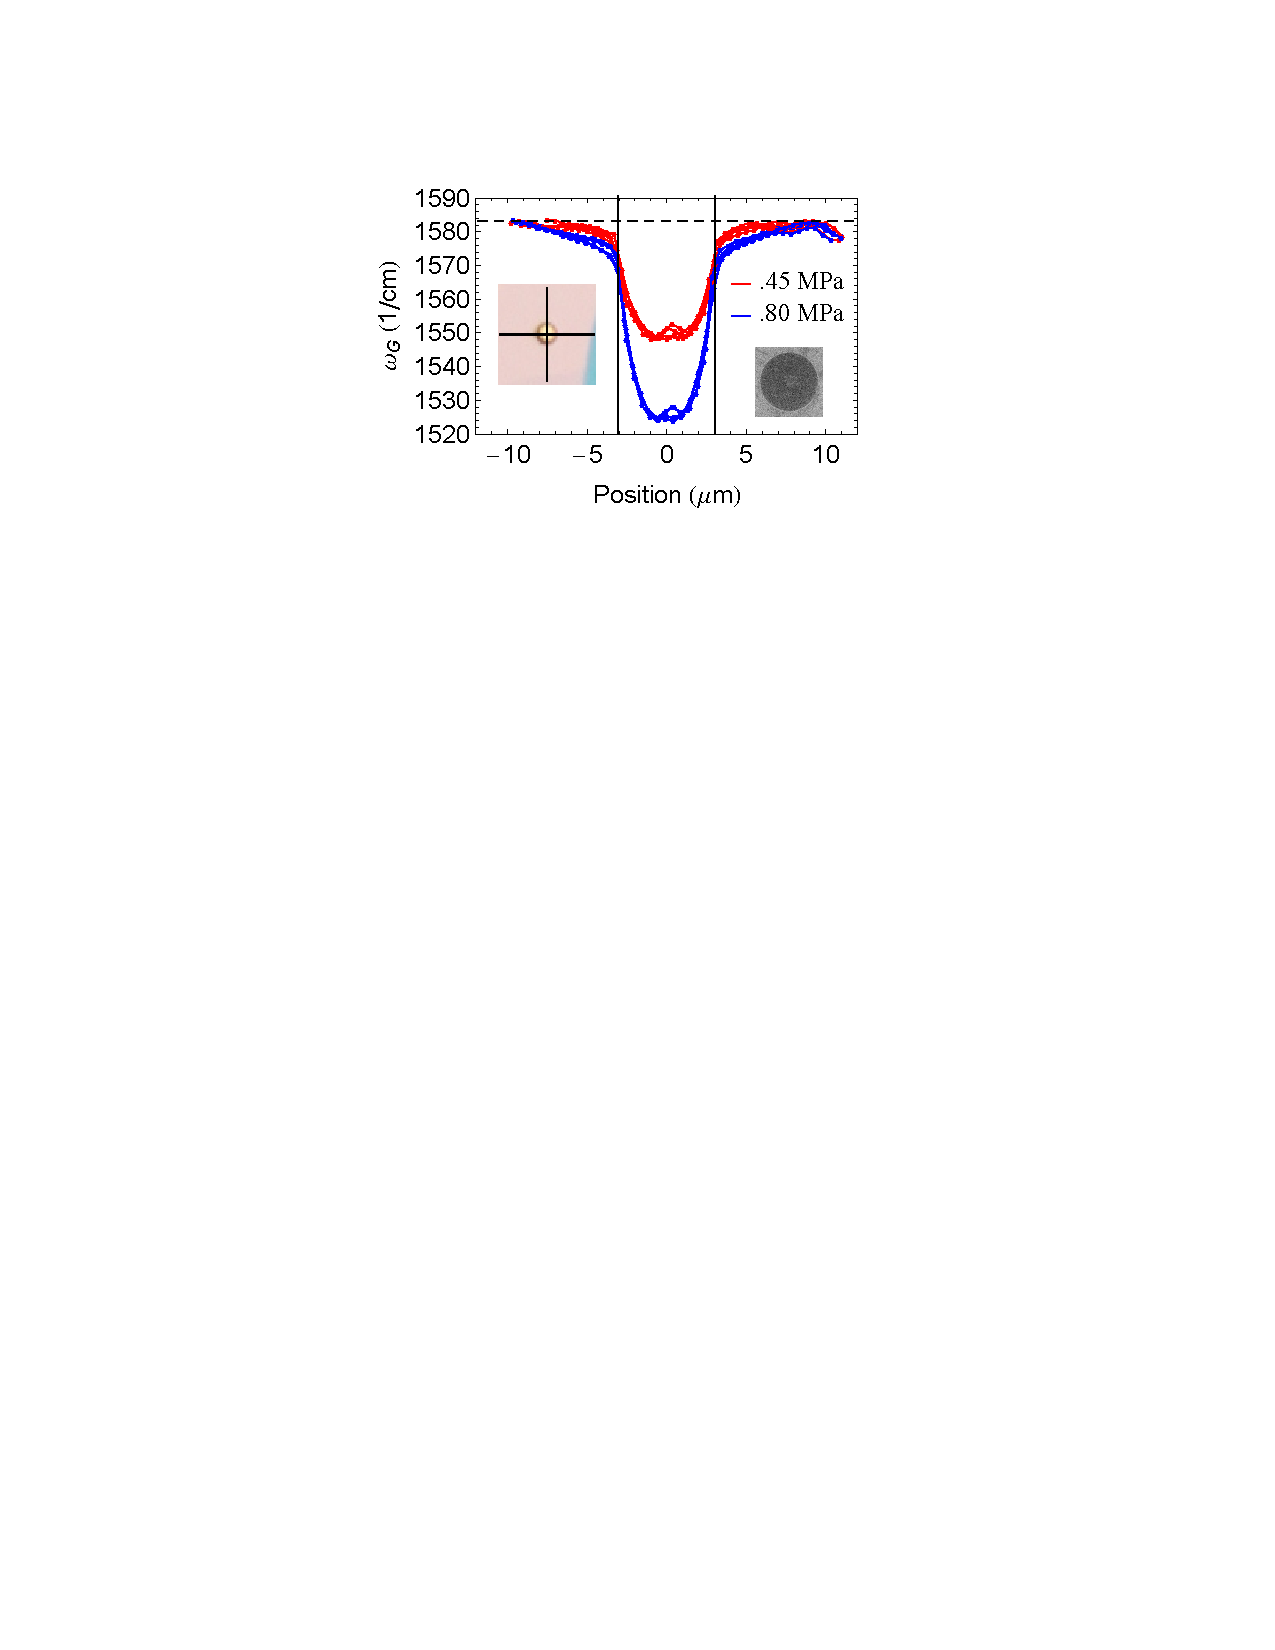
\includegraphics{Figs_Friction/Figure_2.pdf}
\end{center}
\caption{\label{qualresults}The frequency shift of the Raman G band as a function of position for four line scans taken at 0.45 MPa and five line scans taken at 0.80 MPa from 3 separate pressure cycles scanned across a single $6 \ \mu m$ diameter monolayer sealed microchamber. Inset left shows sample and line scan directions.  Each point represents the position of the center of a single Lorentzian fit to the Raman spectra at that position.  Solid vertical black lines are positioned at the edges of the microchamber and the dashed horizontal line indicates the zero strain position of the G band.  Data points are separated by $0.5 \ \mu m$; the focused beam has a waste of $0.81 \ \mu m$.  The bottom right inset is an SEM image of the device after all data acquisition showing the laser induced dirt deposited at the center of the microchamber.}
\end{figure}

To determine the nature of the strain outside of the microchamber, Raman spectra $2 \ \mu m$ outside the edge of a $10 \ \mu m$ diameter monolayer covered microchamber were analyzed in detail.  Circularly polarized spectra at this point show two discrete $G^+$ and $G^-$ peaks confirmed with linearly polarized spectra as shown in Figure \ref{qualout}.  The peak positions indicate a tensile radial strain of 0.6\% and a compressive tangential strain of -0.3\% at this location.  The compressive tangential strain is expected: when an annulus of the supported FLG is pulled inward, its circumference shrinks and, if the adhesion energy between FLG and its substrate is large enough to suppress out-of-plane wrinkling, this shrinkage causes compressive tangential strain.

In our Raman and AFM experiments we see no evidence of the FLG wrinkling to relieve its compressive strain. As shown in Figure \ref{cylindrical}, a partial Raman map of this $10 \ \mu m$ diameter monolayer covered microchamber at 0.80 MPa shows a high degree of radial symmetry indicative of wrinkle free graphene.  To generate the Raman maps shown in Figure \ref{cylindrical}, Raman spectra were taken at each spatial location on the map.  Each spectra was fit with two Lorentzians with energies $\omega^+$ and $\omega^-$ and the best fit energies were plotted as a function of position. The two Lorentzian fit matches the characteristic two peak shape of the supported graphene shown in Figure \ref{circlelinear} for $\rho=1.4$.  Both maps in Figure \ref{cylindrical} were scaled to emphasize the shifts in the supported graphene peak positions.  As a result, the more highly strained suspended graphene appears black in the maps.  The $\omega^-$ Raman map, (a), shows very high radial symmetry while the $\omega^+$ map, (b), has slightly reduced symmetry.  At the highest point on the microchamber, there is a variation of around four wavenumbers in the $\omega^+$ map which could be due to small variations in local adhesion or doping.  The degree of radial symmetry exhibited by both of these Raman maps is a strong indicator that the supported graphene is not wrinkling.  Since these Raman maps are for the microchamber with the largest diameter and thinnest thickness at the highest applied pressure, the compressive strains are the highest of any of the microchambers measured.  Thus, we can rule out wrinkling for our other microchambers which have lower compressive strain.

\begin{figure}
\begin{center}
	\newcommand{\sscale}{.6}
	\newcommand{\sscaler}{.3}
	\begin{tikzpicture}[scale=\sscale]	
		%The picture of the hole with the desciption of phiin and phoout
		\newcommand{\arrowlength}{1 cm}
		\begin{scope}[xshift=-4 cm,yshift=0 cm]
			%The spectra
			\node at (0,0) {\includegraphics[scale=\sscale]{Figs_Friction/PolarForSi.pdf}};
			%The hole
			\newcommand{\hcent}{1 cm}
			\begin{scope}[xshift=-.9 cm,yshift=10.15 cm,>=stealth]
				\node at (0,0) {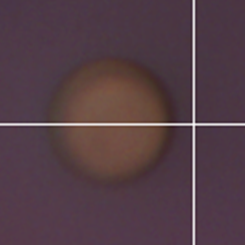
\includegraphics[scale=\sscaler ]{Figs_Friction/PolarPicture.png}};
				\draw[red,ultra thick,->] (\hcent-\arrowlength/2,-.03 cm) -- +(\arrowlength,0)  node[anchor=south west,fill=white]{$\phi_{in}$};
				\draw[green,ultra thick,->] (\hcent,-.03 cm) +(45:-\arrowlength/2) -- +(45:\arrowlength/2) node[anchor=south east, fill=white]{$\phi_{out}$};
			\end{scope}
		\end{scope}
		
		%The figure of the oscillating areas
		\begin{scope}[xshift=4 cm,yshift=0 cm]
			\node at (0,0) {\includegraphics[scale=\sscale]{Figs_Friction/ForSi_Areas.pdf}};
		\end{scope}
		
		\node at (.7,3) {\textbf{b}};
		\node at (-7,12.5) {\textbf{a}};
	\end{tikzpicture}
\end{center}
\caption{\label{qualout} Linearly polarized Raman spectra of supported graphene.  (a) Spectra taken $2 \ \mu m$ outside a $5 \ \mu m$ radius graphene sealed microchamber pressurized to 0.80 MPa absolute pressure with the incident light polarized in the $\hat x$ direction ($\phi=0$) and the outgoing light linearly analyzed from -88 to 92 degrees in 20 degree steps.  The two peaks centered at $1570.9 \ 1/cm$ and $1581.3 \ 1/cm$ are selected by rotating the outgoing analyzer.  (b) The areas under the $1570.9 \ 1/cm$ and the $1581.3 \ 1/cm$ peak are shown as a function of outgoing analyzer angle in black and red, respectively.  The two data sets are fit with $\pi$ out-of-phase sine squared functions illustrating the expected orthogonality of the $G^+$ and $G^-$ peaks\cite{Huang2009}. The peak positions indicate a tensile radial strain of 0.6\% and a compressive tangential strain of -0.3\% at this location.}
\end{figure}

\begin{figure}
\begin{center}
	\begin{tikzpicture}
		\node at (-4.75,2.75+5.5) {\textbf{a:} $\omega^-$};
		\node at (0,5.5) {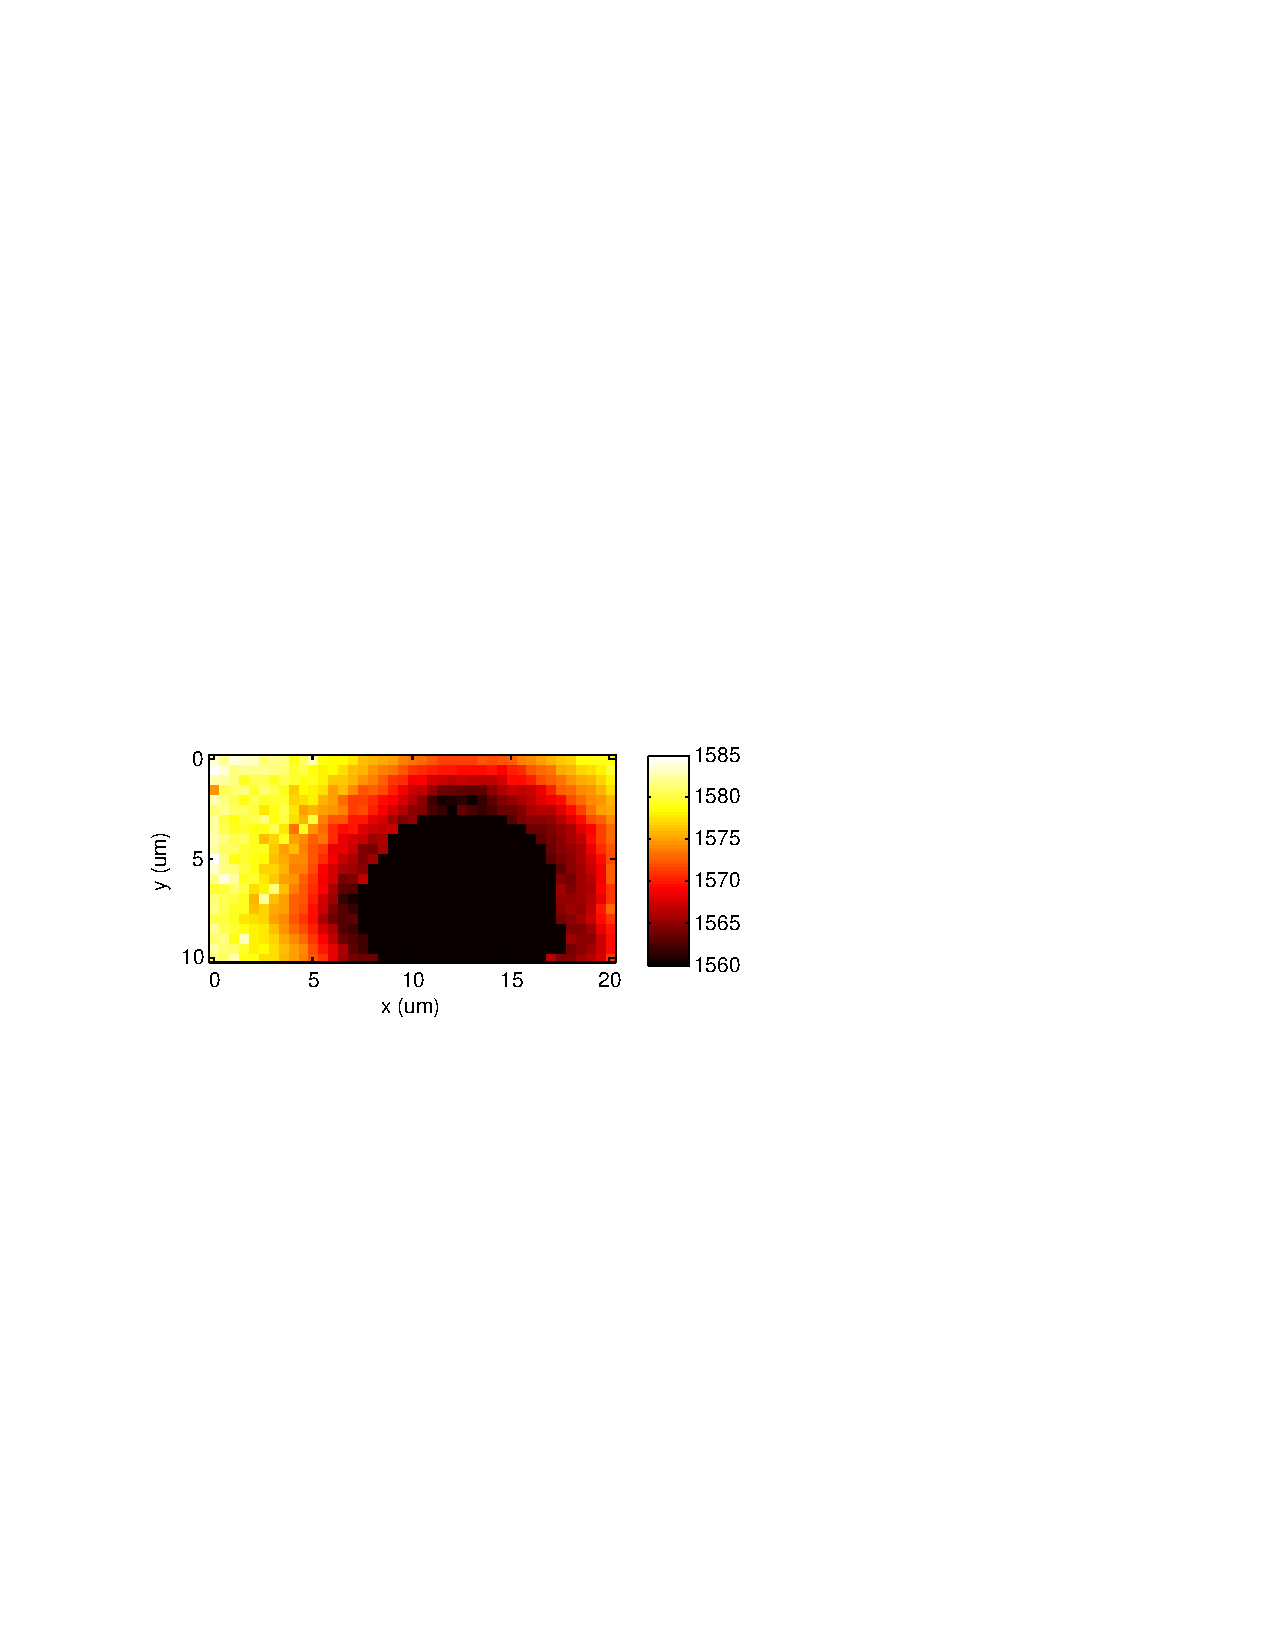
\includegraphics[scale=1]{Figs_Friction/x2.pdf}};
		\node at (-4.75,2.75) {\textbf{b:} $\omega^+$};
		\node at (-.065,-.08) {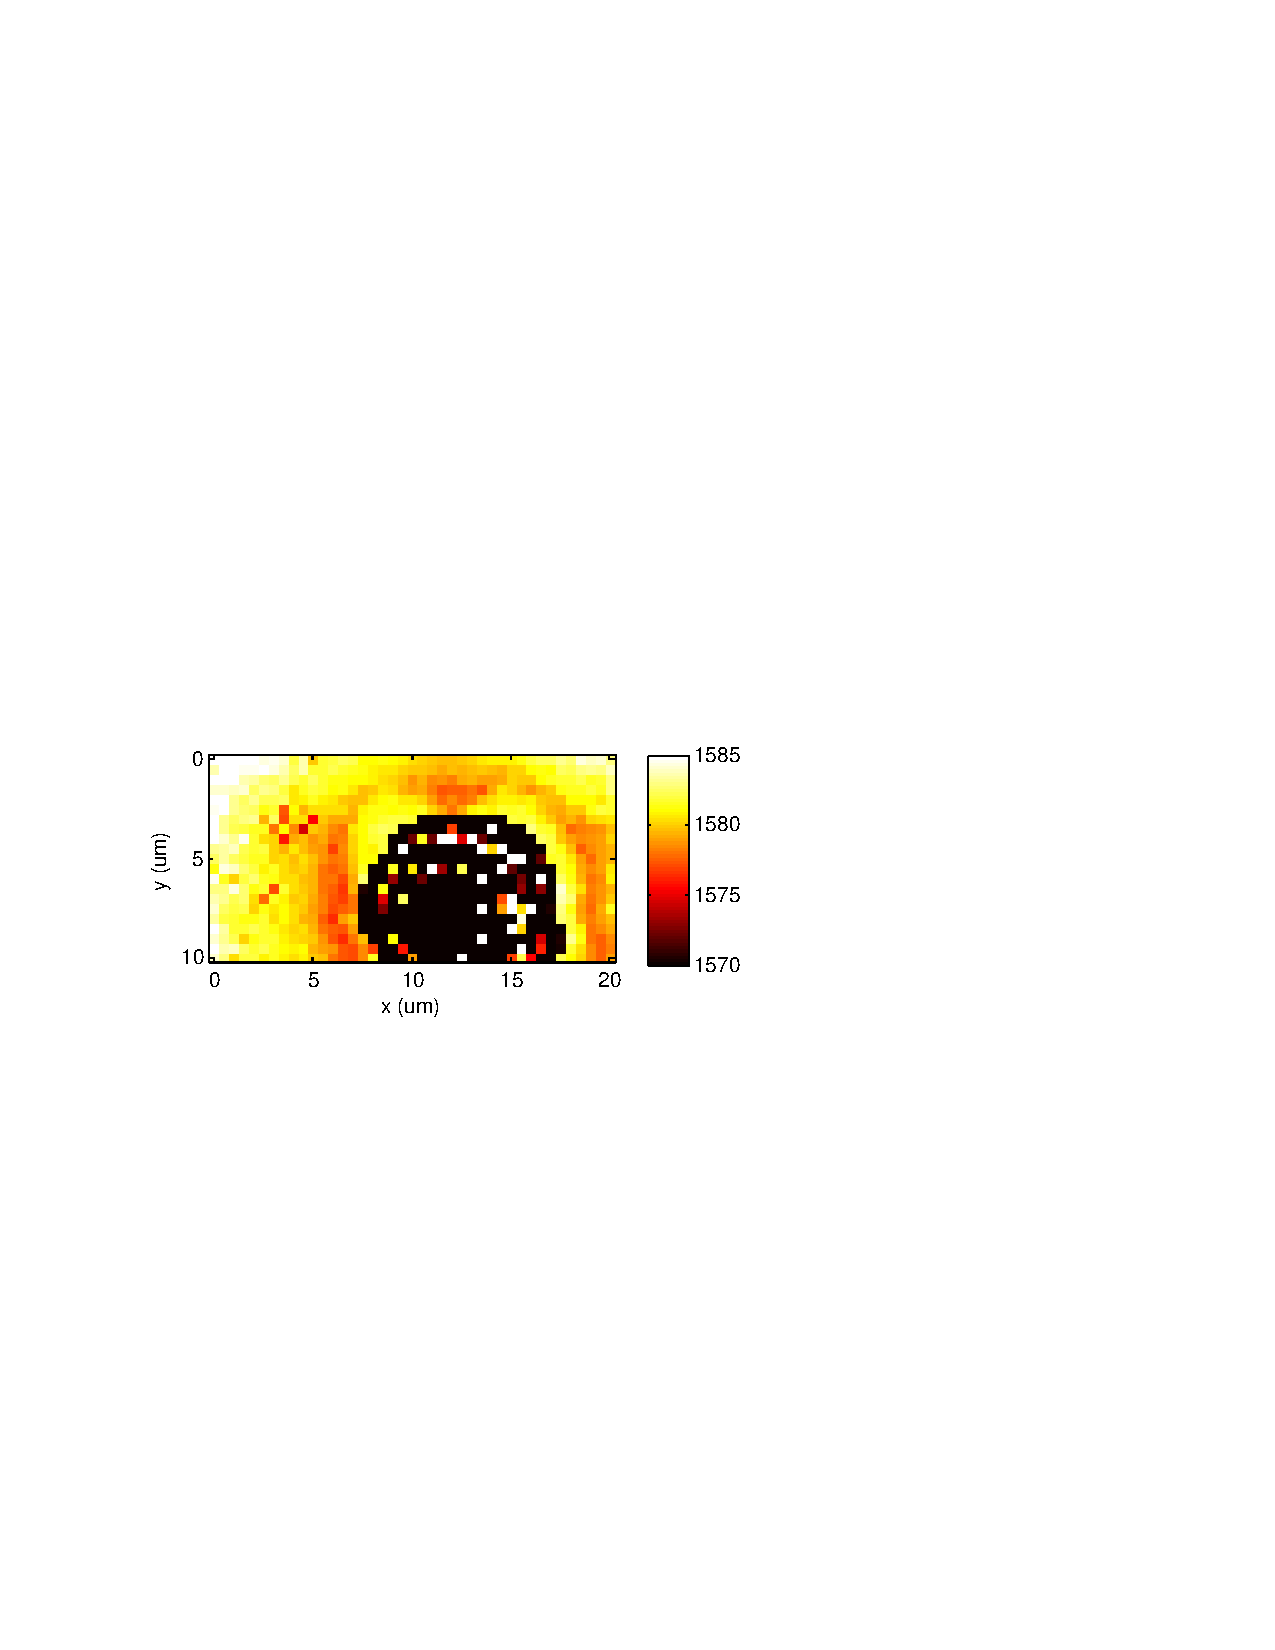
\includegraphics[scale=1]{Figs_Friction/x3.pdf}};
	\end{tikzpicture}
\end{center}
\caption{\label{cylindrical} Raman map of (a) the $\omega^+$ peak and (b) $\omega^-$ peak for a $5 \ \mu m$ radii graphene sealed microchamber pressurized to 0.80 MPa.  In both maps the color scale is set to emphasize the peak shifts experienced by the supported graphene.  The speckles in (b) appear because the suspended graphene spectra are not fit well by two Lorentzians.  Both maps show a high degree of radial symmetry inconsistent with the formation of wrinkles.}
\end{figure}

\section{Continuum model of strain distributions}
We have developed a continuum model to extract the sliding friction, $f$, from the Raman determined strain distributions. In 1915, Hencky proposed a continuum model for the non-linear pressure induced deflection of a thin circular plate with fixed boundary conditions \cite{Hencky1915,Fichter1997}.  This model has been successfully used to describe a variety of systems including inflatable membrane mirrors\cite{Meinel2000}, electrostatic actuators for micro gas pumps\cite{Zhang2011b}, and the topography of FLG bulging from sealed microchambers\cite{Koenig2011}.  The fixed boundary conditions assumed by this model preclude its application to the strain distributions that we observe.  However, we are able to relax the fixed boundary conditions and extend the Hencky model by matching the radial and tangential stresses inside the hole, derived from Hencky's model before the application of boundary conditions, to the radial and tangential stresses of the supported material outside of the hole calculated by including a sliding friction, $f$, acting against the radial displacement.  The stresses and, using Hooke's law, the strains, are then fully determined as a function of $\frac{\Delta P^2 E_{2D}}{f^3 R}$ where $R$ is the radius of the microchamber measured by AFM, $\Delta P$ is the differential pressure, and $E_{2D}$ is the 2D Young's modulus of FLG taken to be $n \times 340 \ N/m$ where n is the number of layers\cite{Lee2008,Koenig2011}.  A full derivation is included in the next section for those interested. Figure \ref{theory} compares the radial and tangential strains from the standard Hencky solution, our extended Hencky solution and an atomistic, molecular dynamics model.  The solid lines of our extended model demonstrate the desired features; strain is distributed \emph{outside} of the hole with compressive tangential, and tensile radial strain. The strain distribution depends on the friction as expected: At constant pressure and radius, a greater sliding friction holds the graphene more firmly to the substrate surrounding the hole, and thereby increases $\epsilon_c$, the strain in the center of the microchamber while also reducing $\rho_0$, the largest radial distance that the strain is acting outside of the hole.  Our extended model, with f=520 MPa, is in good agreement with the dots in Figure \ref{theory} that are the results of an atomistic molecular dynamics simulation of a 6 nm radius microchamber under 500 MPa of pressure performed using the open source simulation package LAMMPS~\cite{plimptonLAMMPS,PlimptonJCP1995} developed at Sandia National Labs.  A detailed description of the atomistic modeling is included below for those interested. To our knowledge, this is the first time that Hencky's model has been generalized to allow strain to be distributed outside of the microchamber's edge.

\begin{figure}
\begin{center}
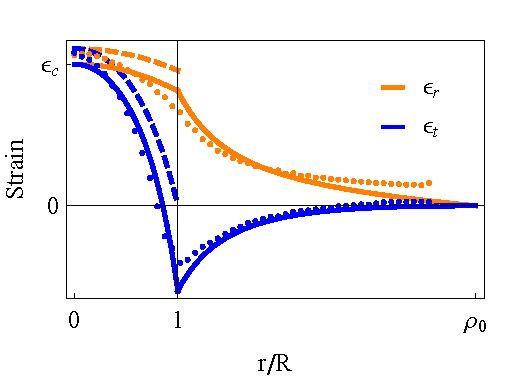
\includegraphics{Figs_Friction/Figure_3.pdf}
\end{center}
\caption{\label{theory} Theoretical strains in few layer graphene sealed microchambers. Comparisons of the radial and tangential strains predicted by Hencky's model (dashed), our extended Hencky model that includes strain outside the microchamber for a sliding friction of f=520 MPa (solid), and atomistic simulations of a 6 nm radius microchamber with 500 MPa of applied pressure (dots). The extended Hencky model used to extract friction agrees very well with the atomistic model.}
\end{figure}

\subsection{Detailed derivation of the extended Hencky model}
Throughout this section we treat graphene in the continuum limit as a thin plate: A solid which is much thinner in one dimension than the other two.  The Hencky model \cite{Hencky1915,Fichter1997} is a series solution for the pressure induced deflection of a thin circular plate with fixed boundary conditions. Here we extend the model to allow strain to be distributed outside of the edges of the hole.  Instead of applying fixed boundary conditions at the edge of the hole, the radial and tangential stresses inside the hole are matched to the radial and tangential stresses experienced by the material being pulled into the hole.  This fully defines the strain in the system as a function of the dimensionless loading parameter, $q=\frac{\Delta PR}{E_{2D}}$, and the dimensionless friction coefficient $F=Rf/E_{2D}$ in the combination $q^{2/3}/F$. Large dimensionless loading, $q^{2/3}$, causes the same effects as  small friction, $F$;  pulling hard has the same effect as sliding easily. Here $\Delta P$ is the pressure differential over the plate, $R$ is the radius of the hole, and $E_{2D}$ is the product of the Young's modulus and the thickness of the plate.  A simple analytic relationship does not exist between  $q^{2/3}/F$ and the two parameters which define the shape of the strain profile: the distance over which the strain spreads outside of the hole, $\rho_0$, and the coefficient of stress at the center of the hole, $b_0$.  However, these can easily be solved for analytically.  To find solutions to our extended Hencky model the general forms of the stress inside and outside of the hole will be derived, and then the boundary condition will be determined and applied.

Assuming that there is no shear, the stress-strain relationship for the thin plate is the same inside and outside the hole\cite{Landau1986}:
\begin{align}
\epsilon_r&=\sigma_r-\nu \sigma_t \label{esr}\\
\epsilon_t&=\sigma_t-\nu \sigma_r \label{est}
\end{align}
where $\nu$ is the Poisson Ratio and $\sigma_r$ and $\sigma_t$ are the dimensionless radial and tangential stresses given by the stress divided by the Young's modulus.

Both the strain-displacement and the governing equations, however, depend on the region of interest. Inside the hole the plate flexes down into the hole as pressure is applied.  The resulting strain-displacement relationships are:
\begin{align}
\epsilon_r^i&=\frac{dU}{d\rho}+\frac{1}{2} (\frac{dW}{d\rho})^2 \label{edri}\\
\epsilon_t^i&=\frac{U}{\rho} \label{edti}
\end{align}
here $U$ is the dimensionless radial deflection, $W$ is the dimensionless out of plane deflection, and $\rho$ is the dimensionless radius, all of which are made dimensionless by dividing by the radius of the hole.   The governing equations inside the hole are calculated by balancing the forces on a radial element.  The stresses and pressure acting on such an element are shown in Figure \ref{stressfigurei}.
\begin{figure}
\begin{center}
	\begin{center}
	\newcommand{\halfangle}{10}
	\begin{tikzpicture}[scale=2]
	%The radial equilibrium
	\begin{scope}[xshift=-4.5 cm]
		%The bisected dotted lines
		\begin{scope}[dashed,gray,very thin]
			\draw (0,0) -- (\halfangle:1.5 cm);
			\draw (0,0) -- (-\halfangle:1.5 cm);
		\end{scope}
		%Draw the area element
		\filldraw[fill=gray!10,draw=black] (-\halfangle:1.5 cm)  arc(-\halfangle:\halfangle:1.5 cm) -- (\halfangle:2 cm) arc(\halfangle:-\halfangle:2 cm) -- cycle;
		%Draw the force lines and labels
		\begin{scope}[->, blue!50!black,>=stealth]
			\draw (0:2 cm) -- +(0:.25 cm) node[anchor=west]{$N_r+\frac{dN_r}{dr} dr$};
			\draw (0:1.5 cm) -- +(0:-.25 cm) node[anchor=east]{$N_r$};
			\draw (\halfangle:1.75 cm) -- +(90+\halfangle:.25 cm) node[anchor=south east]{$N_t$};
			\draw (-\halfangle:1.75 cm) -- +(-90-\halfangle:.25 cm) node[anchor=north east]{$N_t$};
		\end{scope}
		\draw (.25,.75 cm) node{Top:};
	\end{scope}
	
	%The lateral equilibrium
	\begin{scope}[->, blue!50!black,>=stealth]
		\draw (0,0) -- (20:-.25 cm) node[anchor=north east]{$N_r$};
		\draw[black,thick,-] (20:0 cm) -- ++(20:.5 cm);
		\draw (20:.5 cm)  -- ++(20:.25 cm) node[anchor=west]{$N_r+\frac{dN_r}{dr} dr$};
		\draw (20:.25 cm) -- ++(90:.25 cm) node[anchor=west]{$P$};
		\filldraw (0,0) circle(.5pt);
		\filldraw (20:.5 cm) circle(.5pt);
		\filldraw (20:.25 cm) circle(.5pt);
	\end{scope}
	\draw (-.25,.75 cm) node{Side:};
	
	\end{tikzpicture}
	\end{center}
\caption{\label{stressfigurei}The stresses, $N_r$ and $N_t$, and pressure, $P$ acting on a radial area element for $\rho<1$ as viewed from the top and side.}
	\end{center}
\end{figure}
Using the area of the radial element ($r dr d\theta$) to convert the pressure to a force, and the cross sectional area to convert the strains into forces results in the two governing equations:
\begin{align}
\sigma_t^i&=\frac{d}{d \rho}(\rho \sigma_r^i) \label{g1i}\\
\sigma_r^i \frac{dW}{d \rho}&=-\rho \frac{q}{2} \label{g2i}
\end{align}
the first from radial equilibrium and the second from lateral equilibrium with $\sigma_r$ and $\sigma_t$ the radial and tangential stresses, $N_r$ and $N_t$, divided by the Young's modulus to make them dimensionless.  These six equations can be combined to form a single differential equation for $\sigma_r$:
\begin{equation}
\frac{1}{8} \rho q^2+ (\sigma_r^i)^2 \frac{d}{d\rho}[\sigma_r^i+\frac{d}{d\rho}(\rho \sigma_r^i)]=0
\label{comboin}
\end{equation}
This is most easily found by using eqn. \ref{g1i} and then eqn. \ref{g2i} in the combination of equations: $[(\ref{edri}) \rightarrow (\ref{esr})]-\frac{d}{d \rho}\rho[(\ref{edti})\rightarrow(\ref{est})]$.  Solving this equation for $\sigma_r$ determines $\sigma_t$, $\epsilon_r$, and $\epsilon_t$ using equations \ref{g1i}, \ref{esr}, and \ref{est}.  Since there is no analytic solution to this differential equation, we follow Hencky and assume a series expansion of the radial stress even in powers of $\rho$ to match symmetry:
\begin{equation}
\sigma_r^i=\frac{1}{4} q^{2/3} \sum_{n=0}^{\infty} b_{2n} \rho^{2n}
\end{equation}
When used in eqn. \ref{comboin} all of the higher order coefficients are determined in terms of one free parameter, $b_0$, the stress coefficient at the center of the hole.  To this point the derivation has not deviated from Hencky's original work.  However, instead of continuing forward to determine the value of $b_0$ by requiring that there is no radial deflection at the edge of the hole, $b_0$ will be left as a free parameter to match to the strain outside of the hole, which we now derive.

Outside of the hole the plate is constrained to move in the x-y plane, radial symmetry is preserved, and friction is present.  The stress strain relationships (eqns. \ref{esr} and \ref{est}) are for a thin plate with no shear, and thus, apply equally well outside the hole as inside.  The strain displacement relationships are based on the geometry of a general radially symmetric differential element.  The only change that needs to be made to these is the elimination of the out of plane motion:
\begin{align}
\epsilon_r^o&=\frac{dU}{d\rho} \label{edro}\\
\epsilon_t^o&=\frac{U}{\rho} \label{edto}
\end{align}
For sufficiently negative $\epsilon_t$, the plate is expected to buckle out-of-plane, forming wrinkles.  However, in our experimental regime we do not see evidence for these effects.  The forces acting on the plate are different inside and outside the hole, and thus, so are the governing equations.  The stresses and forces acting on the graphene outside of the hole are shown in Figure \ref{stressfigureo}.
\begin{figure}
\begin{center}
	\begin{center}
	\newcommand{\halfangle}{10}
	\begin{tikzpicture}[scale=2]
	%The bisected dotted lines
	\begin{scope}[dashed,gray,very thin]
		\draw (0,0) -- (\halfangle:1.5 cm);
		\draw (0,0) -- (-\halfangle:1.5 cm);
	\end{scope}
	%Draw the area element
	\filldraw[fill=gray!10,draw=black] (-\halfangle:1.5 cm)  arc(-\halfangle:\halfangle:1.5 cm) -- (\halfangle:2 cm) arc(\halfangle:-\halfangle:2 cm) -- cycle;
	%Draw the force lines and labels
	\begin{scope}[->, blue!50!black,>=stealth]
		\draw (0:2 cm) -- +(0:.25 cm) node[anchor=west]{$N_r+\frac{dN_r}{dr} dr$};
		\draw (0:1.5 cm) -- +(0:-.25 cm) node[anchor=east]{$N_r$};
		\draw (\halfangle:1.75 cm) -- +(90+\halfangle:.25 cm) node[anchor=south east]{$N_t$};
		\draw (-\halfangle:1.75 cm) -- +(-90-\halfangle:.25 cm) node[anchor=north east]{$N_t$};
		\filldraw[red!40!black] (1.75,0) circle(.5pt);
		\draw[red!40!black] (1.75,0) -- +(.15,0) node[anchor=south east]{$f$};
	\end{scope}
	\end{tikzpicture}
	\end{center}
\caption{\label{stressfigureo}The stresses, $N_r$ and $N_t$, and friction, $f$, on a radial area element for $\rho>1$.}
	\end{center}
\end{figure}
The interaction between the plate and its underlying substrate is included via the frictional force per unit area, $f$, which is pointed to oppose the stresses outside of the hole.  Care needs to be taken in this mathematical treatment because this friction term does not turn off when the stress goes to zero.  Instead, it works in positive feedback amplifying the stress.  As a result, the stresses are only physical until they decay to zero at a position $\rho_0$.  If there were a component of friction acting against the tangential strain, it would go as $d \theta^2$, one power for the resultant and one power for the area element, rendering it negligible.  The governing equation outside the hole is then:
\begin{equation}
\sigma_t^o=\frac{d}{d\rho}(\rho \sigma_r^o)+F \rho
\label{g1o}
\end{equation}
Again these equations can be combined to form a single differential equation for $\sigma_r$.  The easiest way to do this is by using eqn. \ref{g1o} twice in the combination of equations: $[(\ref{edro}) \rightarrow (\ref{esr})]-\frac{d}{d \rho}\rho[(\ref{edto})\rightarrow(\ref{est})]$.  The result is:
\begin{equation}
\frac{d}{d\rho}[\sigma_r^o+\frac{d}{d\rho}(\rho \sigma_r^o)]=-(2+\nu) F
\label{comboout}
\end{equation}
Unlike the situation inside of the hole, this equation can be solved exactly.  The general result for the radial and tangential stress (eqn. \ref{g1o}) are:
\begin{align}
\sigma_r^o&=(2+\nu)F(-\frac{\rho}{3}-\frac{c_2}{2 \rho^2})+c_1 \\
\sigma_t^o&=(2+\nu)F(-\rho \frac{1+2 \nu}{3(2+\nu)}+\frac{c_2}{2 \rho^2})+c_1
\end{align}
Usually, it would be natural to restrict this solution by requiring that the strain at $\rho=\infty$ goes to zero.  In this case, this cannot be done because of the unphysical form of the strain for positions $\rho>\rho_0$.  Instead, the radial and tangential strains are forced to both go to zero at the position $\rho_0$.  This gives $c_2=\rho_0^3 \frac{\nu-1}{3(2+\nu)}$ and $c_1=\rho_0 \frac{1+\nu}{2} F$, completely defining the strains outside in closed form as a function of one free parameter, $\rho_0$, which defines the furthest reach of the stress outside of the hole.

Having determined the stresses inside and outside of the hole, the boundary condition for the stresses at the edge of the hole will be determined.  The stress is related to the force per unit area through a divergence operation:
\begin{equation}
F_i=\frac{\partial N_{ik}}{\partial x_k}
\end{equation}
where $F_i$ is the force per unit volume in the $i$ direction, $N_{ik}$ is the strain tensor, and repeated indices are summed over.  Integrating the equations and using the divergence theorem gives:
\begin{equation}
\int_V F_i \ dV=\oint_S \sigma_{ik} \ df_k
\end{equation}
The total force acting on a volume entity is given by the surface integral of the stress.  A symmeterized volume element that spans the edge of the hole is shown in Figure \ref{egestress}.  In the limit that $\epsilon \rightarrow 0$ the distributed surface forces $f$ and $P$ contribute nothing to the force on this volume element, forcing the left hand side to zero. This would not be the case if these were 1D edge forces. The undrawn tangential stresses also go to zero as the cross section that they act on, $\epsilon h$, goes to zero as well.  Thus, the remaining stresses must be equal:
\begin{equation}
N_r^i=N_r^o
\end{equation}
The boundary condition on the tangential stress is found by the requirement that the radial displacement, $U$, must be continuous.  If it were not, the material on one side of the discontinuity would separate from the material on the other side leaving a gap.  If $U$ is continuous, so must $\epsilon_t$ be by eqns. \ref{edti} and \ref{edto}.  Finally, if $\epsilon_t$ and $N_r$ are continuous, so must $N_t$ be by equation \ref{est}.  Thus, we have shown that the radial and tangential stresses must be continuous over the edge of the hole.


\begin{figure}
\begin{center}
	\begin{center}
	\newcommand{\halfangle}{10}
	\newcommand{\dr}{.3 cm}
	\newcommand{\rbeg}{1.5 cm}
	\newcommand{\Larrow}{.25 cm}
	\begin{tikzpicture}[scale=2]
	%The bisected dotted lines
	\begin{scope}[dashed,gray,very thin]
		\draw (0,0) -- (\halfangle:\rbeg);
		\draw (0,0) -- (-\halfangle:\rbeg);
	\end{scope}
	%Draw the area element
	\filldraw[fill=gray!10,draw=black] (-\halfangle:\rbeg)  arc(-\halfangle:\halfangle:\rbeg) -- (\halfangle:\rbeg+\dr) arc(\halfangle:-\halfangle:\rbeg+\dr) -- cycle;
	%Draw the edge of the hole
	\draw[dotted,thick] (-4*\halfangle:\rbeg+\dr/2) arc(-4*\halfangle:4*\halfangle:\rbeg+\dr/2) node[anchor=south]{$\rho=1$};
	%Draw the force lines and labels
	\begin{scope}[->, blue!50!black,>=stealth]
		\draw (0:\rbeg+\dr) -- +(0:\Larrow) node[anchor=west]{$N_r^o$};
		\draw (0:\rbeg) -- +(0:-\Larrow) node[anchor=east]{$N_r^i$};
		\filldraw[red!40!black] (\rbeg+\dr*3/4,0) circle(.5pt);
		\draw[red!40!black] (\rbeg+\dr*3/4,0) -- +(.1,0) node[anchor=south east]{$f$};
		\filldraw[red!40!black] (\rbeg+\dr*1/4,0) circle(.5pt) node[anchor=north]{$P$};
	\end{scope}
	%Draw the width of the element
	\draw[<->,black,>=stealth] (\halfangle*5/4:\rbeg) -- node[anchor=south]{$\epsilon \rightarrow 0$} +(\halfangle*5/4:\dr);
	\end{tikzpicture}
	\end{center}
\caption{\label{egestress}The stresses and forces acting on a thin, symmetrized volume element which spans the edge of the hole.  The tangential strains inside and outside are ignored as their contribution goes to zero as $\epsilon \rightarrow 0$.}
	\end{center}
\end{figure}

With a series solution for the stresses inside the hole with the stress at the center of the hole, $b_0$, as a free parameter, and with a closed form solution for the stresses outside of the hole with the furthest distance the stress spreads, $\rho_0$, as a free parameter, we can match the stresses with the boundary condition to uniquely define the stresses in terms of $q$ and $\mu$. We use the continuity of the radial and tangential stresses at the boundary to solve for our two free parameters $\rho_0$ and $b_0$.
\begin{align*}
\sigma_r^i(\rho=1)&=\sigma_r^o(\rho=1) \\
\sigma_t^i(\rho=1)&=\sigma_t^o(\rho=1) 
\end{align*}
This sets the value of $\rho_0$ and $b_0$ in terms of $q^{2/3}/F$.  Regrettably, the series form of the solution inside of the hole makes the presentation of an exact expression for $\rho_0$ and $b_0$ impossible.  Numerical solutions for the values of $\rho_0$ and $b_0$ are presented in Figures \ref{rho0} and \ref{b0} for graphite's Poisson ratio of 0.165\cite{Blakslee1970}.  As the friction increases or the dimensionless loading coefficient decreases, $q^{2/3}/F$ decreases, and $\rho_0$ decreases toward unity, the value for no strain distribution outside of the hole, while $b_0$ increases toward 1.66, the result of the Hencky model. 

\begin{figure}
\begin{center}
\begin{center}
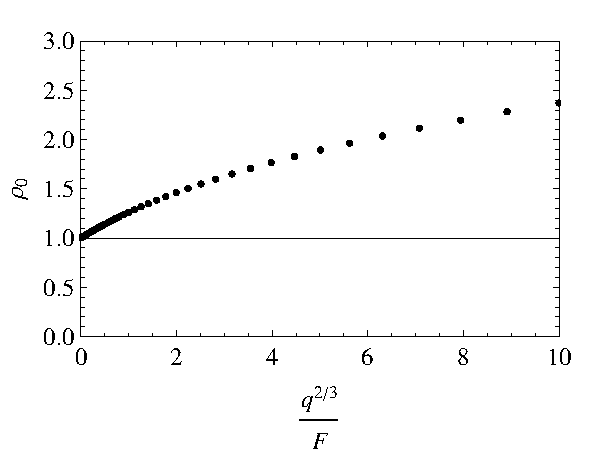
\includegraphics{Figs_Friction/rho0.pdf}
\end{center}
\end{center}
\caption{\label{rho0} Numerical solutions for values of $\rho_0$. Note convergence to $\rho_0 = 1$ as the dimensionless loading decreases or the friction increases, corresponding to no stress distributed outside of the hole.}
\end{figure}

\begin{figure}
\begin{center}
\begin{center}
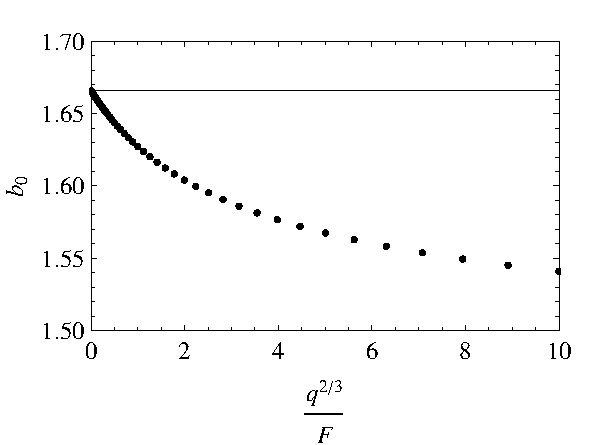
\includegraphics{Figs_Friction/b0.pdf}
\end{center}
\end{center}
\caption{\label{b0} Numerical solutions for values of $b_0$. Note the convergence to the value 1.66 for small loading (or large friction), approaching the result of the Hencky model.}
\end{figure}

\subsection{Detailed derivation of Atomistic model}
Classical molecular dynamics simulations (MD) were performed using open source simulation package LAMMPS~\cite{plimptonLAMMPS,PlimptonJCP1995} developed at Sandia National Labs to investigate the atomistic details underlying the experimental results. The model used argon gas to compress a graphene monolayer that lies atop an amorphous silicon dioxide substrate, as illustrated in Figure \ref{MD}.  The substrate had dimensions 46 x 46 x 3 nm with a 6 nm radius hole in the center.  A circular graphene monolayer with radius 22 nm was placed on top of the hole in the substrate and argon atoms were randomly distributed within the simulation box after relaxation of the graphene-substrate system.   There were 562,110 atoms in total, with the simulation run in parallel for maximum computational efficiency.

The covalent carbon bonds were modeled using the AIREBO\cite{stuartJCP2000} potential, which has been shown to have good accuracy in describing hydrocarbon systems~\cite{qiNANO2010,zhaoJAP2010}.  The Tersoff~\cite{tersoffPRB1988} potential was utilized for the Si-Si, Si-O and O-O interactions, while a Lenard-Jones potential was used for all other interactions with a cutoff distance of 8\AA \ and the corresponding interaction parameters chosen as follows: $\epsilon_{Ar-Ar}$=0.0104eV, $\sigma_{Ar-Ar}$=3.405\AA~\cite{RytkonenJchemp1998}; $\epsilon_{Ar-C}$=0.0123eV, $\sigma_{Ar-C}$=3.573\AA~\cite{RobertNano1996};$\epsilon_{Ar-Si}$=0.0028eV, $\sigma_{Ar-Si}$=3.778\AA~\cite{LiPRA2010}; $\epsilon_{Ar-O}$=0.0058eV, $\sigma_{Ar-O}$=3.3075\AA~\cite{EverittJCP1999}; $\epsilon_{Si-C}$=0.008909eV, $\sigma_{Si-C}$=3.326\AA~\cite{OngPRB2010}; $\epsilon_{O-C}$=0.003442eV, $\sigma_{O-C}$=3.001\AA~\cite{OngPRB2010}.  The Ar-Si and Ar-O interaction parameters were obtained using the standard Lorentz-Berthelot mixing rule.

\begin{figure}
\begin{center} \begin{center}
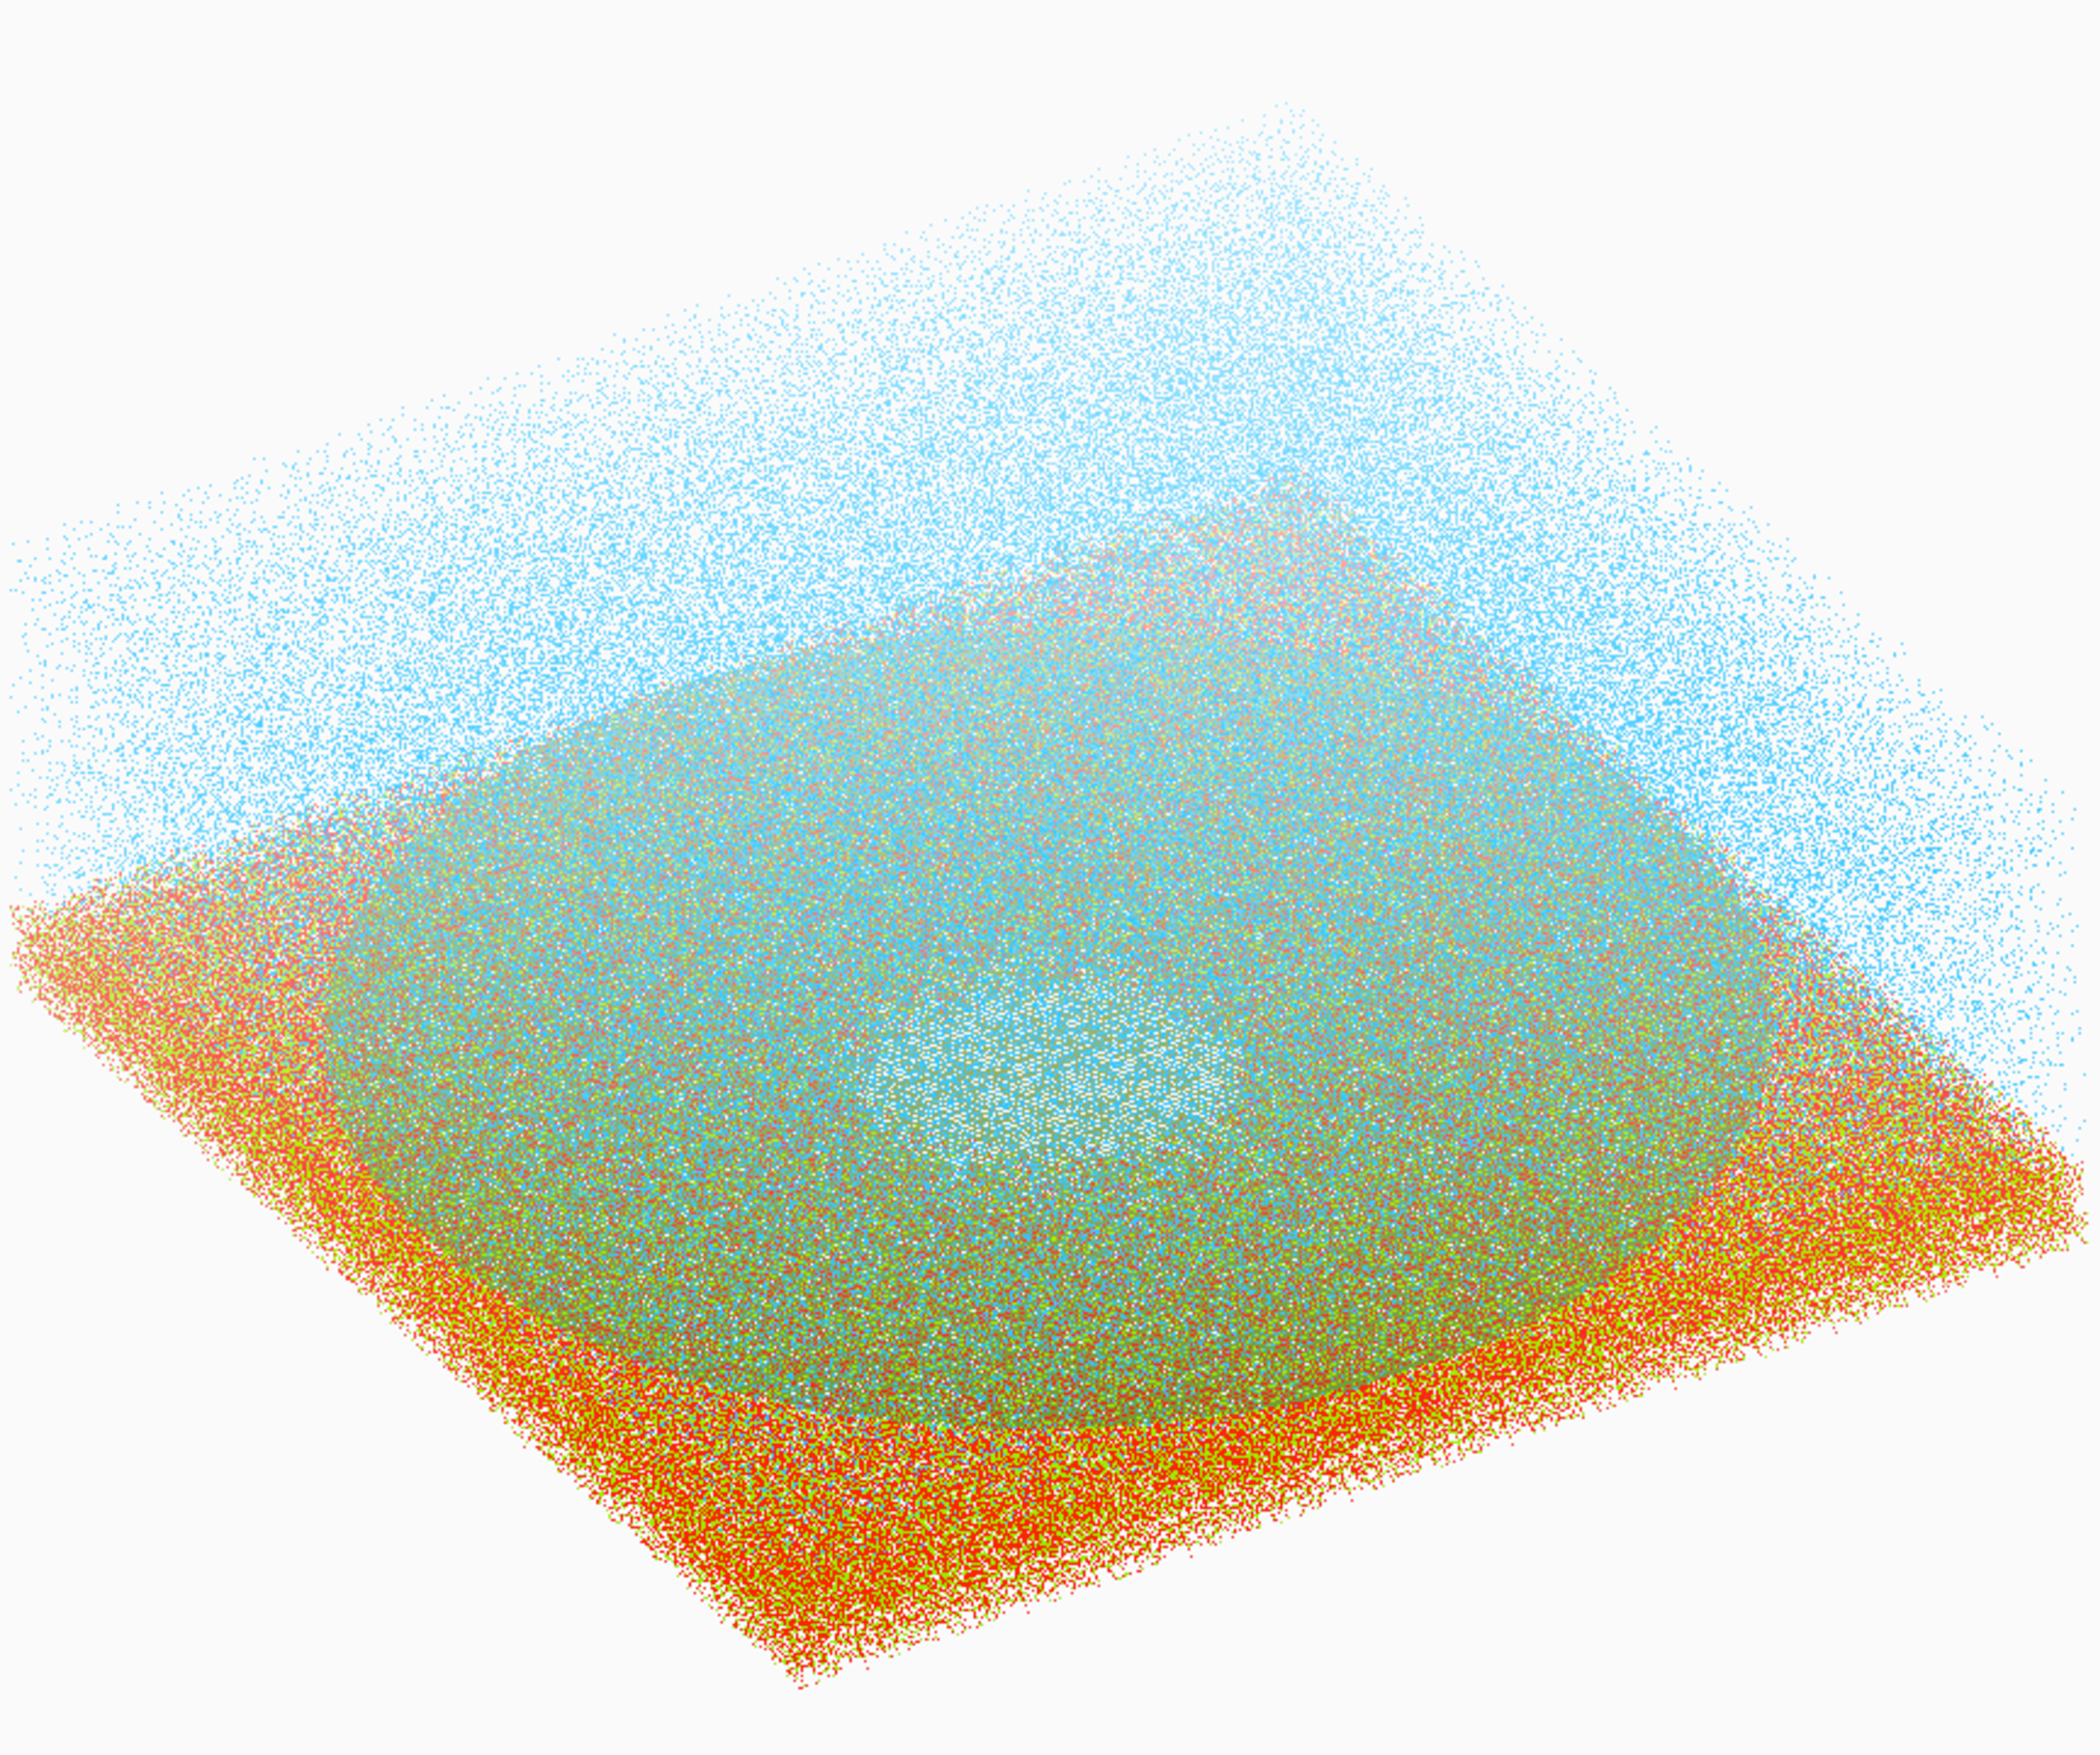
\includegraphics[scale=0.15]{Figs_Friction/MD.pdf}
\end{center}
\caption{\label{MD} Schematic diagram of the simulation system including (from bottom to top) amorphous SiO$_{2}$ substrate (red and orange atoms), circular graphene monolayer (brown atoms) and argon gas (cyan atoms). Visualization was performed using Visual Molecular Dynamics~\cite{Humphrey1996}.}
 \end{center} \end{figure}

The system was first relaxed at room temperature (300K) for .03 MPa, at which point the gas density was slowly increased by reducing the volume of gas to increase the pressure.  When the desired deflection of graphene was reached, the gas density was then kept fixed, and the system was allowed to relax at that pressure for 10 ps.  The final equilibrium configuration of graphene was computed by averaging over all of the atomic positions of graphene during the relaxation period with constant gas density. The substrate was assumed to be rigid and fixed during the simulation.  As a boundary condition on the graphene, the atoms in the outer 1 nm annulus of the supported graphene were fixed during the simulation matching the experimental observation that the supported graphene only slides in a local region around the hole, remaining fixed at large radii.  A canonical ensemble (NVT) with room temperature (300K) was used for the entire simulation and reflection boundary conditions were used to ensure that gas atoms remained inside the simulation box.  

To calculate the strain in the deformed graphene sheet, we first calculated the atomistic displacement field~\cite{ZimmermanIJSS2009} by calculating the difference between the reference (initial) configuration and the final, deformed configuration.  The strain tensor from continuum mechanics was then calculated as
\begin{equation} \label{eq:straindisp}
\epsilon_{ij}=\frac{1}{2}\left(\frac{\partial {u_i}}{\partial {X_j}} + \frac{\partial {u_j}}{\partial {X_i}} + \frac{\partial{u_k}\partial{u_k}}{\partial{X_i}\partial{X_j}}\right),
\end{equation}
where $\epsilon_{ij}$ are the components of the strain, $u$ is the displacement, and $X$ denotes the position of a point in the reference configuration.

The displacement field $\mathbf{U}$ for each atom was computed by linearly interpolating, using standard finite element method shape functions for triangular elements~\cite{hughes1987}. The displacements of its three nearest neighbors as $\mathbf{U}=\mathbf{N}\bullet\mathbf{u_N}$, where $\mathbf{N}$ are the finite element shape functions and $\mathbf{u}_{N}$ are the displacements for each atom.  From the displacement field $\mathbf{U}$, the strain was calculated by taking derivative of $\mathbf{U}$ as $\mathbf{\epsilon}=\mathbf{B}\bullet\mathbf{u_N}$, where $\mathbf{B}=\frac{\partial \mathbf{N}}{\partial \mathbf{X}}$. The atomistic data plotted in the paper was obtained from the MD simulation results by the method above, and was expressed in polar coordinates. 

\section{Fitting Raman spectra to the continuum model}
The extended continuum model can be used to analyze the measured Raman spectra to determine the sliding friction as well as the Gr\"{u}neisen parameter and shear deformation potential.  Comparing the extended Hencky model to strains found by directly inverting the positions of the $G^+$ and $G^-$ peaks is not possible because of the finite size of the focused laser beam.  Instead, the strains predicted by the extended Hencky model are convoluted with the system point spread function to predict an entire group of Raman G band line scan spectra for different sets of values of the fitting parameters.  The set of parameters that minimize the global $\chi^2$ is chosen as the best fit to the data.

 Errors in the fitted parameters found by using the increase in $\chi^2$ away from its minimum value\cite{Press2007} are better than one part in one hundred, much smaller than we can claim to have achieved in our experiment.  This discrepancy is due to an underestimation of our uncertainties which include only photon counting and ignore effects due to inhomogeneous doping, sample drift, and laser assisted deposition of dirt on the FLG.  To better illustrate the relative uncertainties amongst different fitted friction values we use a 0.25 increase of $\chi^2$ per degree of freedom above the best fit value to define confidence intervals.  The width and position of the unstrained G band for supported FLG is taken from the spectra at the largest radial distance measured during a line scan at either 0.17 MPa or atmospheric pressure, while the G band width for the suspended graphene is taken from the center of the atmospheric pressure line scan.

 When fitting the extended Hencky model to the measured spectra, for microchambers with radii larger than $1.2 \ \mu m$ the global $\chi^2$ includes every spectra in the line scan except for those located less than half the beam waist away from the edge of the microchamber.  This is done to avoid including the additional fitting parameters needed to account for the signal mismatch between suspended and supported FLG created by different optical interference conditions.  When fitting the smaller radius microchambers ($R<1.2 \ \mu m$), the spectra from the suspended graphene are ignored. Figure \ref{igouter} shows an example of the resulting best fit.  Spectra from the suspended region ($\rho<1$) exhibit a high energy shoulder that is not predicted by the extended Hencky model.  This feature is observed in each of the three graphene sealed microchambers with radius less than $1.2 \ \mu m$ but not for the five larger radius microchambers.  We believe this feature arises from airy rings in the focused laser beam.  These rings of intensity would contribute signal from lower strain regions giving a distinct higher energy signal, and not a broadening.  For larger radius microchambers, the laser spot is smaller relative to the microchamber radius and so it samples a more uniform distribution of strains, making an extra contribution from the airy rings unimportant. Complications of fitting these features are avoided by only including the spectra from the supported graphene when fitting.  

\begin{figure}
\begin{center}
	\begin{tikzpicture}[scale=.675]
		%The spectra
		\node at (0,0) {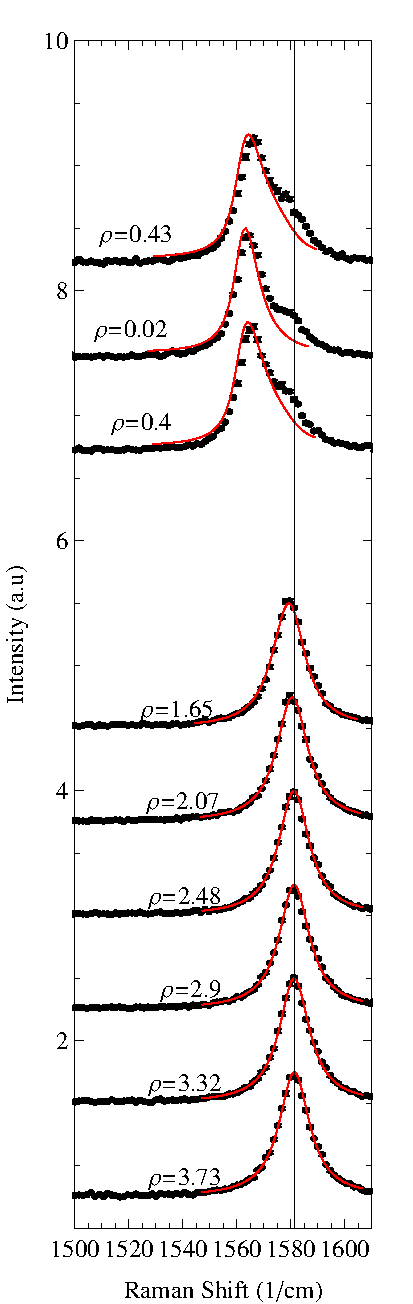
\includegraphics[scale=.675]{Figs_Friction/2012-12-18_Fit_101psi_Spectra_for_paper_sb04-6b.pdf}};
		
		%The picture of the hole
		\newcommand{\arrowlength}{.144*2.4 cm}%.144 is 2.5 um
		\begin{scope}[xshift=-.5 cm,yshift=1.25 cm]
			%For the total scale=1 the .jpg scale is .6
			\node at (0,0) {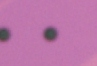
\includegraphics[scale=.30375,angle=-90]{Figs_Friction/SB04-6b.jpg}};%was .225 before I change the scale from .5 to .45
			\draw[->,black,>=stealth] (-.03cm,-\arrowlength-.05 cm-.136 cm) -- +(0,2*\arrowlength);
		\end{scope}
	\end{tikzpicture}
\end{center}
\caption{\label{igouter} Global fitting details for microchambers with radii less than 1.2 microns. Raman spectra from a line scan over a $\sim 1.2 \ \mu m$ radius bilayer sealed microchamber with 0.80 MPa of applied absolute pressure. The spectra taken along the path shown in the lower left inset are arrayed vertically with those spectra that were too close to the edge of the hole to be fit omitted.  The black vertical line is positioned at the supported graphene's unstrained G band energy.  The value of the sliding friction was found by fitting the spectra of the supported graphene ($\rho>1$) only.  Plotted in red are the spectra predicted by our extended Hencky model using the best fit to the sliding friction.  Even though they were not included in the fit, the spectra predicted by the extended Hencky model matches the major feature of the suspended spectra. }
\end{figure}

Unlike the sliding friction, the Gr\"{u}neisen parameter and shear deformation potential should be the same for every line scan.  As such, they were included as fitting parameters only in the two lines scans which best defined the shear deformation potential based on the splitting of the supported graphene's G band just outside the edge of the microchamber: the $\sim 5 \mu m$ radius monolayer and the $\sim 5 \mu m$ radius trilayer at 0.80 MPa of applied pressure.  The best fit values, $\gamma=1.89 \pm 0.01$ and $\beta=0.70 \pm 0.04$, were then treated as known material parameters for the rest of the twenty full Raman line scans.  Figure \ref{gammabeta} details the extraction of these parameters.  Table \ref{gb} summarizes the measurements of the Gr\"{u}neisen parameter and shear deformation potentials of other research groups as well as their substrates.  Our measured $\gamma$ is commensurate with most of the other measured values and agrees particularly well with the \textit{ab initio} calculations of Cheng \emph{et al.}\cite{Cheng2011}.  On the other hand, our measured shear deformation potential is lower than most other measurements.  Buckling out-of-plane cannot explain this result since the mono and trilayers would buckle differently for a microchamber with the same pressure and radius. To our knowledge, these are the first measurements of $\gamma$ and $\beta$ for which the sliding of FLG over its substrate was included.

\begin{figure}
\begin{center}
	\newcommand{\sscale}{.8}
	\begin{tikzpicture}[scale=\sscale]	
		\begin{scope}[xshift=-4.5 cm,yshift=0 cm]
			\node at (0,0) {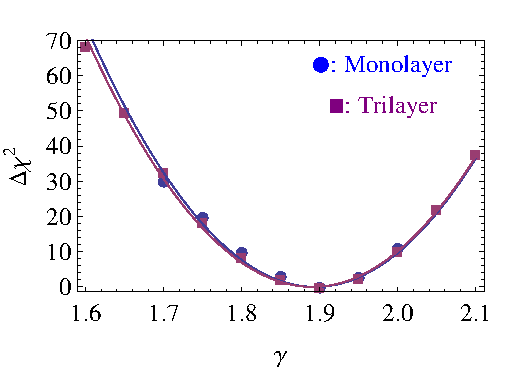
\includegraphics[scale=\sscale]{Figs_Friction/2012-12-11_Gbest.pdf}};
			\node at (-3.8,3) {\textbf{a}};
		\end{scope}
		
		\begin{scope}[xshift=4.5 cm,yshift=0 cm]
			\node at (0,0) {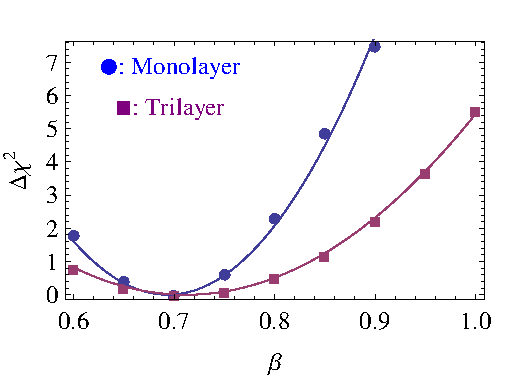
\includegraphics[scale=\sscale]{Figs_Friction/2012-12-11_Bbest.pdf}};
			\node at (-3.8,3) {\textbf{b}};
		\end{scope}
	\end{tikzpicture}
\end{center}
\caption{\label{gammabeta}Determination of the Gr\"{u}neisen parameter and shear deformation potential. Global fits to a monolayer covered and a trilayer covered $\sim 5 \ \mu m$ radius sealed microchamber at 0.80 MPa of applied absolute pressure are used to determine the Gr\"{u}neisen parameter, $\gamma$, and shear deformation potential, $\beta$. The plotted circles and squares represent the increase of $\chi^2$ per degree of freedom away from the minimum value of the fit with the other fitting parameters ($\beta$ and $f$ for $\gamma$, and $\gamma$ and $f$ for $\beta$) chosen to minimize $\chi^2$ at each data point. The plotted curves represent a parabolic fit to the data. Using an increase in $\chi^2$ per degree of freedom of 0.25 gives: $\gamma_{mono} = 1.89 \pm .02$, $\gamma_{tri} = 1.89 \pm .02$, $\beta_{mono} = 0.69 \pm .04$, and $\beta_{tri} = 0.71 \pm .06$. The averages of the monolayer and the trilayer give $\gamma=1.89 \pm .01$ and $\beta= 0.70 \pm .04$.}
\end{figure}

\begin{table}
\begin{center}
\begin{tabular}{l c  c }
\hline
\hline
 & $\gamma$ & $\beta$ \\
 \hline
 This work & 1.89 & .70 \\
 $\mathrm{SiO_2}$ depression\cite{Metzger2010} & 2.4 & \\
 On PDMS\cite{Huang2009} & .69 & .38 \\
 On SU8\cite{Mohiuddin2009} & 1.99 & .99\\
 Embedded\cite{Frank2010} & 2.01 & 1.01 \\
 On Acrylic\cite{Yoon2011} & 2.2 & .93\\
 Bubble\cite{Zabel2012} & 1.8 \\
\textit{Ab initio} \cite{Thomsen2002} & 2.0 & 0.66 \\
\textit{Ab initio} \cite{Cheng2011} & 1.86 & .96\\
 \hline
 \hline
\end{tabular}
\end{center}
\caption{\label{gb} Summary of the Gr\"{u}neisen parameter, $\gamma$, and shear deformation potential, $\beta$, as measured on different substrates}
\end{table}

Figure \ref{fitlinescan} shows a global data fit for a $\sim 5 \ \mu m$ radius monolayer covered graphene sealed microchamber at 0.80 MPa of applied pressure.  The spectra and fits from each position along the line scan are stacked vertically in the direction of the line scan.  Our extended continuum model successfully fits the softening and splitting of the G band of the supported graphene and successfully predicts the downshift and sharpening of the G band of the suspended graphene as the center of the microchaber is approached. In comparison, without our theoretical extension the standard Hencky model would fail to reproduce the supported graphene spectra.

\begin{figure}
\begin{center}
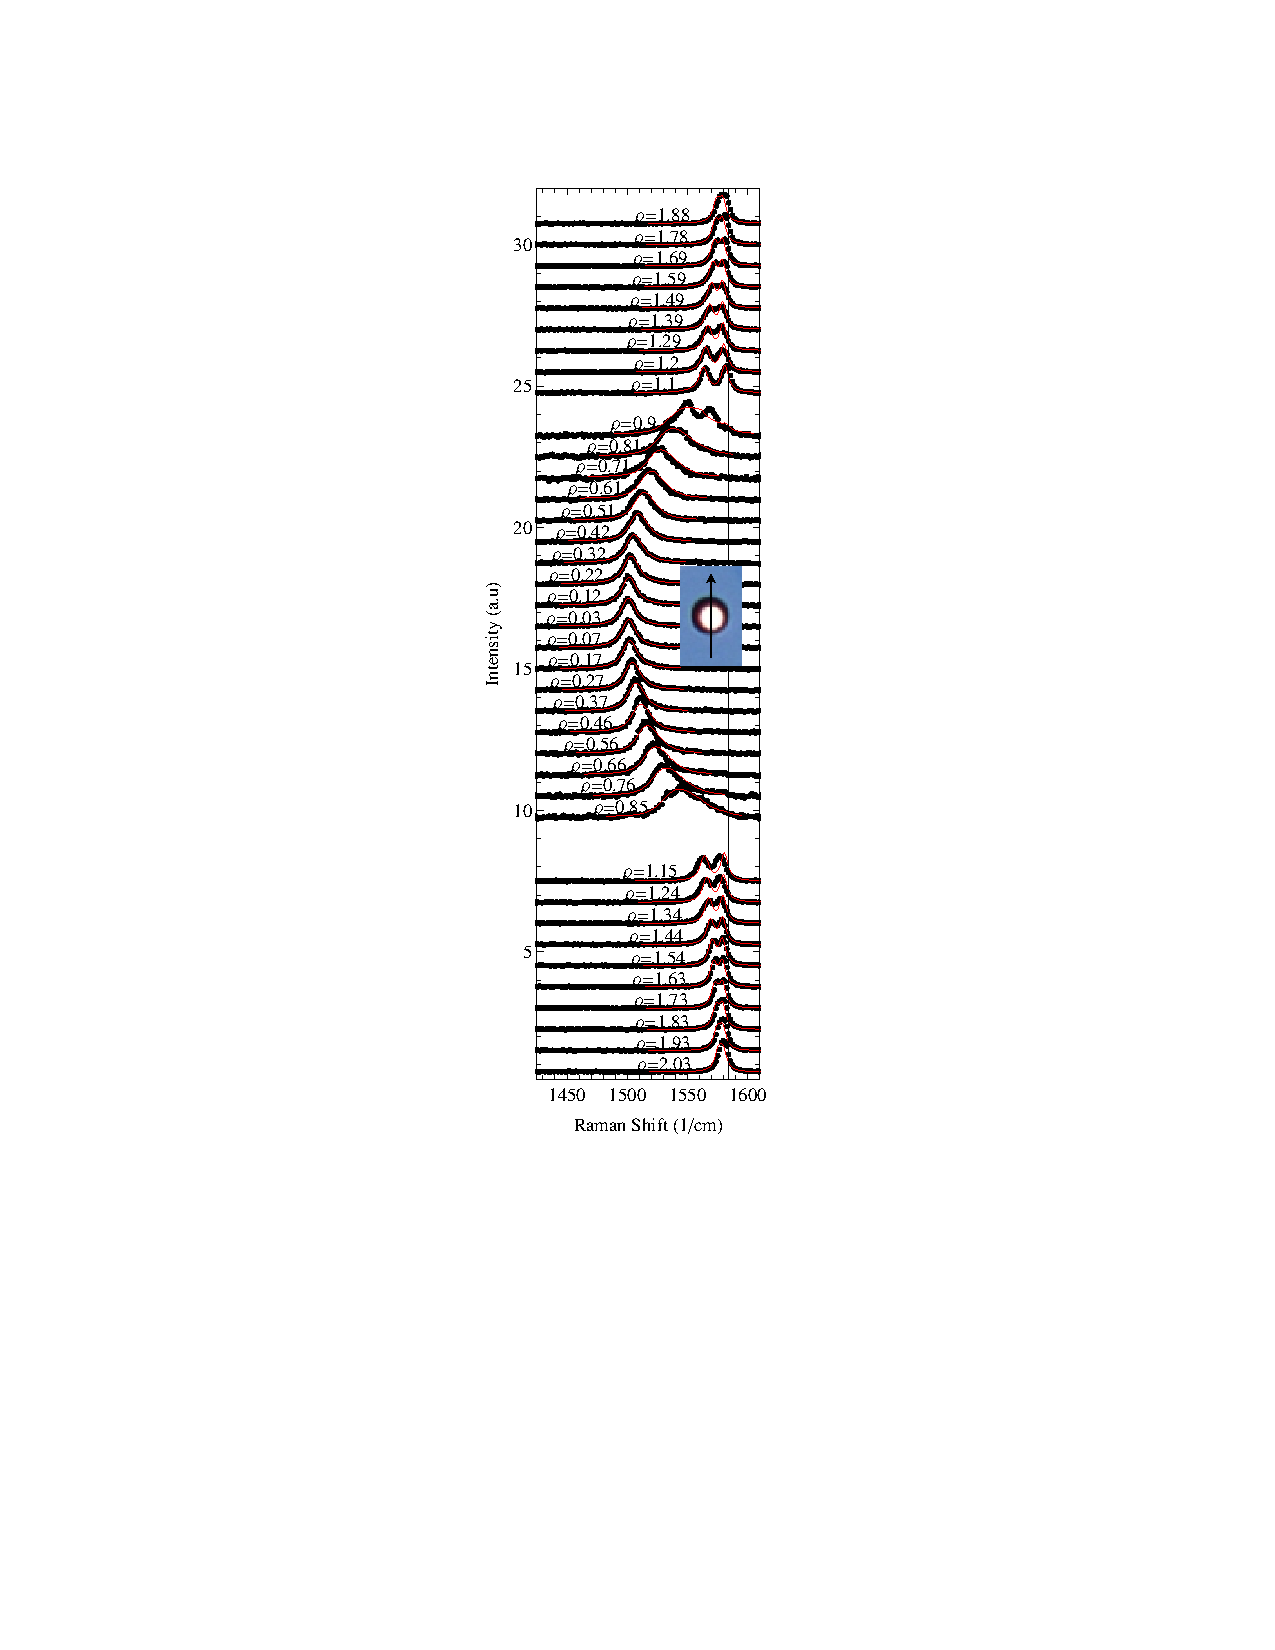
\includegraphics{Figs_Friction/Figure_4.pdf}
\end{center}
\caption{\label{fitlinescan} Raman spectra from a line scan over a $\sim 5 \ \mu m$ radius monolayer graphene sealed microchamber with 0.80 MPa of applied pressure analyzed with our extended Hencky model (red lines).  The spectra taken along the path shown in the inset are arrayed vertically with spectra taken too close to the edge of the microchamber omitted (see text).  The black vertical line is positioned at the supported graphene's unstrained G band energy.}
\end{figure}

\section{Measured frictional dependencies}
The sliding friction extracted for eight microchambers with radii between 1.2 and 5 $\mu m$ and with applied absolute pressures from 0.10 to 0.80 MPa exhibits fundamentally different behavior for trilayer graphene than for monolayer and bilayer.  In Figure \ref{FvsP}a (left) the friction is plotted as a function of pressure and the data for trilayer graphene (black dots) shows a linear dependence of the sliding friction vs applied pressure in accordance with Amontons' law with a coefficient of friction of $0.11 \pm 0.01$ as shown in Figure \ref{trimu}.  The sliding friction for monolayer and bilayer graphene decreases generally with applied pressure and the wide scatter of the points for different radii and layer number clearly indicate that the sliding friction is dependent on the geometry of the microchamber. Our theoretical analysis shows that the radial strain at the edge due to the pressure pushing the graphene into the microchamber has the same radii and layer number dependence as the friction, so we replot the sliding friction as a function of the radial strain in Figure \ref{FvsP}b (right). The monolayer and bilayer data for all different radii microchambers now \emph{collapse} to a single curve versus radial strain, well described by $1/\epsilon_{r,edge}$ behavior (dashed line). 

\begin{figure}
\begin{center}
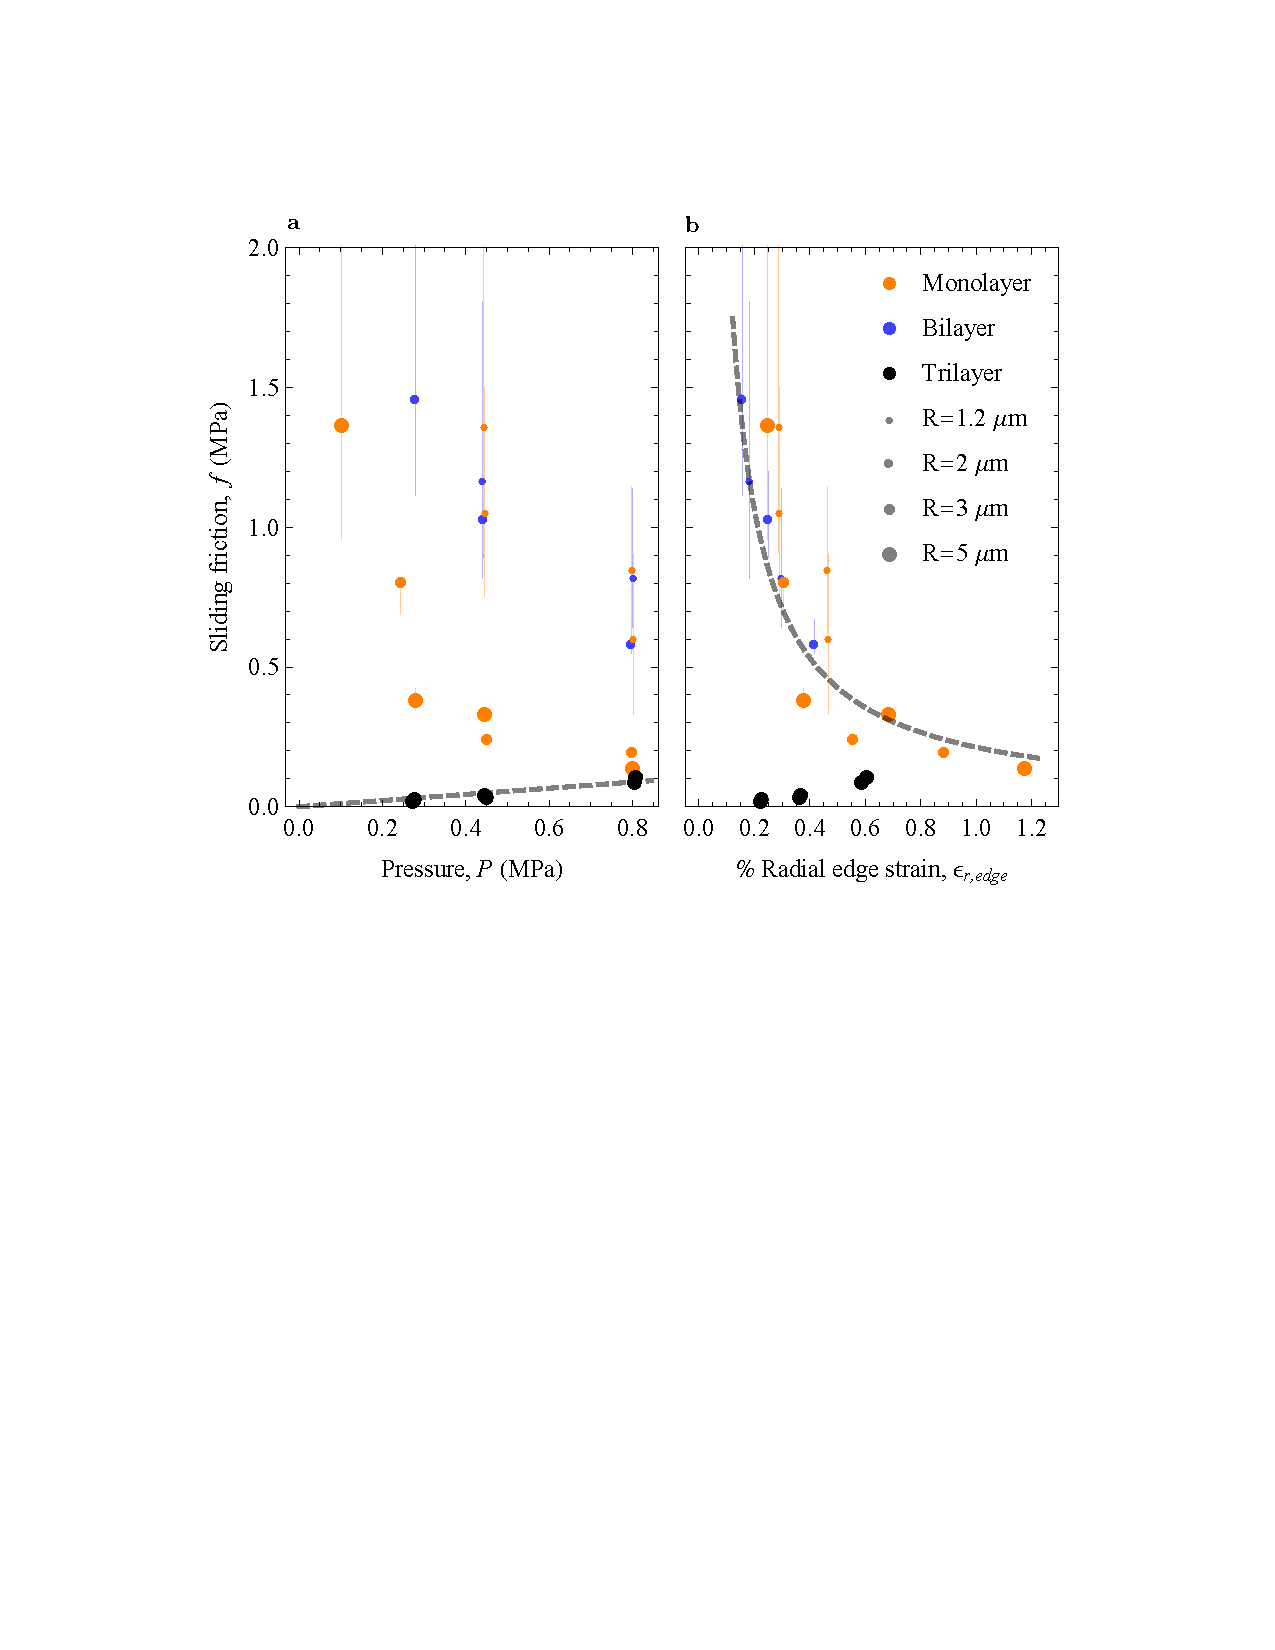
\includegraphics{Figs_Friction/Figure_5.pdf}
\end{center}
\caption{\label{FvsP}  Sliding friction, extracted by analyzing Raman G band line scans with our extended Hencky model, plotted as a function of absolute applied pressure in panel \textbf{a} (left) and as a function of the radial strain at the edge of the microchamber in panel \textbf{b} (right) for 5 different graphene sealed microchambers.  The size of each data point represents the radius of the FLG-sealed microchamber corresponding to that point. The error bars are given by an increase in global fit $\chi^2$ per degree of freedom of 0.25.  The sliding friction of trilayer graphene depends linearly on the absolute applied pressure in agreement with Amontons' law. The sliding friction of monolayer and bilayer graphene, however, go as the inverse of the radial strain at the edge of the microchamber.  Gray dashed lines are the best fits to these trends.}
\end{figure}

\begin{figure}
\begin{center}
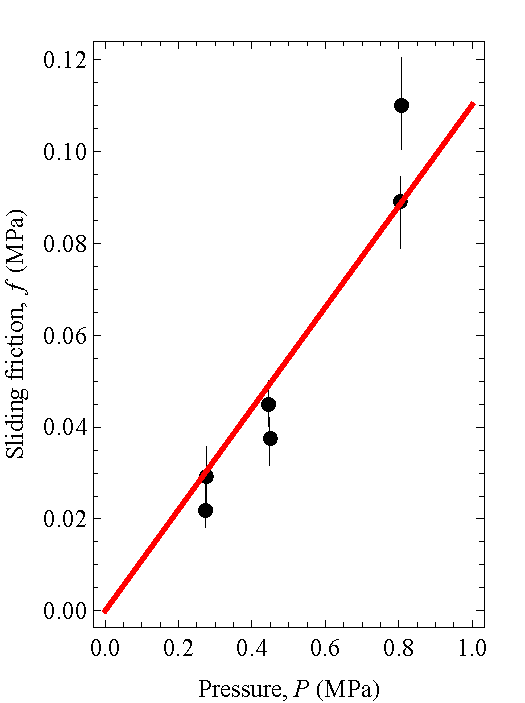
\includegraphics{Figs_Friction/Tri_mu.pdf}
\end{center}
\caption{\label{trimu} Determination of the coefficient of friction for trilayer graphene on silicon dioxide.  The sliding frictions extracted from Raman G band lines scans over two $5 \ \mu m$ radii trilayer sealed microchambers as a function of the absolute applied pressure is fit with Amonton's law, $f=\mu P_{abs}$, giving a coefficient of friction between trilayer graphene and $\mathrm{SiO_2}$ of $\mu=0.11 \pm 0.01$. For reference, Teflon on Teflon has $\mu=0.04$ while clean steel on clean steel has $\mu=0.6$\cite{Resnick2002}.}
\end{figure}

The gross difference in behavior between trilayer on one hand, and mono-and bilayer on the other, illustrates the two roles of the applied pressure. The pressure load pushes the graphene more firmly onto the substrate so that sliding friction should increase (Amontons' law), yielding a positive coefficient of friction. This is the case for the trilayer graphene.  On the other hand, as the pressure pushes the graphene into the microchamber, it creates a radial tension in the supported graphene outside the microchamber. The data collapse in Figure \ref{FvsP}b for monolayer and bilayer graphene demonstrate that the pressure dependence of the sliding friction is not due to loading the supported graphene but is instead due to the graphene being pulled and stretched by the applied pressure.  This is the only mechanism that would depend on the geometric parameters of the microchamber while also being consistent with the data. It is not surprising that the sliding friction for mono- and bilayer graphene is dependent on the strain and not the load because thin graphene conforms nearly perfectly to a $\mathrm{SiO_2}$ substrate\cite{Stolyarova2007,Lui2009,Cullen2010}.  Increasing the load cannot further increase the contact area, but increasing the radial strain beyond the edge of the microchamber may act to smooth out the graphene sheet, decreasing the contact between the graphene and the substrate, and thus decreasing the sliding friction.  The bending rigidity, which goes as thickness cubed, of trilayer graphene must be high enough to counteract the adhesion energy, causing lower conformation and allowing for a traditional pressure and load response. The existence of a bilayer to trilayer crossover in FLG-substrate interactions is also observed in GPa range pressure measurements of silicon dioxide supported graphene\cite{Proctor2009,Nicolle2011}.  Nicolle \emph{et al.} observed a decrease in the pressure response of the G band between bilayer and trilayer graphene which was attributed to the transition from biaxial compression mediated by the substrate to hydrostatic compression mediated by the pressure transmitting medium\cite{Nicolle2011}.

\section{Summary}
In summary, we have shown that graphene slides along the substrate when pulled.  Furthermore, using a newly developed extension of the continuum Hencky model, we extracted the sliding friction as a function of the number of atomic layers and the load.  Trilayer graphene shows a typical load response whereas the sliding friction for monolayer and bilayer graphene goes as the inverse of strain. The data collapse of the friction for mono- and bilayer graphene when plotted versus strain is strong experimental evidence for a reduction in surface conformation when graphene is pulled as the fundamental origin of the negative coefficient of friction.  These results will be important for the design of strain engineered devices\cite{Pereira2009a}, while the sliding of a flexible surface along a bulk object should be of fundamental, tribological interest. Finally, the method used in generalizing Hencky's solution should be useful for including distributed strains in other continuum models for use in designing strain-engineered graphene devices and in understanding other, few-layer material systems.